\documentclass[twoside,11pt,a4paper]{scrbook}

%%%%%%%%%%%%%%%%%%%%%%%%%%%%%%%%%%%%%%%%%%%%%%%%%%%%%%%%%%%%%%%%%%%%5
%%% Packages

\usepackage{geometry}
\usepackage[utf8]{inputenc}
\usepackage[T1]{fontenc}
\usepackage[pdftex]{graphicx}
\usepackage[ngerman]{babel}
\usepackage{colortbl}
\usepackage{soul}
\usepackage{textcomp}
\usepackage[usenames,dvipsnames]{xcolor}
\usepackage[toc,page]{appendix}
\usepackage{amssymb}
\usepackage{amsmath}
\usepackage{enumerate}
\usepackage{tikz}
\usepackage[hidelinks]{hyperref}
\usepackage{lastpage}
\usepackage{nameref}
\usepackage{etoolbox}
\usepackage[binary-units=true]{siunitx}
\usepackage{eurosym}
\usepackage{wrapfig}
\usepackage{multirow,bigdelim}
\usepackage{multicol}
\usepackage{pgfplots}
\usepackage{listings}
\usepackage{array}
\usepackage[within=none]{caption}
\usepackage{adjustbox}
\usepackage{xspace}
\usepackage[inline]{enumitem}
\usepackage{booktabs}
\usepackage{tabularx}
\usepackage{subcaption}
% \usepackage{float}
\usepackage{titlesec}
\usepackage[backend=biber,labelnumber,defernumbers=true,style=authoryear,natbib=true]{biblatex}
\usepackage{makecell}
\usepackage{minted}
\usepackage{nicefrac}
\usepackage{csquotes}
\usepackage{lipsum}
\usepackage{rotating}
\usepackage{pdflscape}
\usepackage{afterpage}
\usepackage{ltablex}
\usepackage{keycommand}

\let\tmp\oddsidemargin
\let\oddsidemargin\evensidemargin
\let\evensidemargin\tmp
\reversemarginpar

% rubber: setlist arguments --shell-escape
%%%%%%%%%%%%%%%%%%%%%%%%%%%%%%%%%%%%%%%%%%%%%%%%%%%%%%%%%%%%%%%%%%%%5
%%% Helper macros for different types of TODOs

\newcommand{\factcheck}{\textcolor{orange}{\textsuperscript{\textbf{!!}}}~}
\newcommand{\citationneeded}{\textcolor{blue}{\textsuperscript{\textbf{??}}}~}
\newcommand{\cn}{\citationneeded} % alias for \citationneeded
\newcommand{\todo}{\textcolor{green}{TODO!}}

%%%%%%%%%%%%%%%%%%%%%%%%%%%%%%%%%%%%%%%%%%%%%%%%%%%%%%%%%%%%%%%%%%%%5
%%% References

\newcommand{\figlabel}[1]{\label{fig:#1}}
\newcommand{\chaplabel}[1]{\label{chap:#1}}
\newcommand{\seclabel}[1]{\label{sec:#1}}
\newcommand{\tablabel}[1]{\label{tab:#1}}
\newcommand{\subseclabel}[1]{\label{subsec:#1}}
\newcommand{\lstlabel}[1]{\label{lst:#1}}

\newcommand{\figref}[1]{\figurename~\ref{fig:#1}}
\newcommand{\chapref}[1]{\chaptername~\ref{chap:#1}}
\newcommand{\secref}[1]{\secname~\ref{sec:#1}}
\newcommand{\tabref}[1]{\tablename~\ref{tab:#1}}
\newcommand{\subsecref}[1]{\subsecname~\ref{subsec:#1}}
\newcommand{\lstref}[1]{\listingscaption~\ref{lst:#1}}

\newcommand{\Figref}[1]{\figref{#1} ,,\nameref{fig:#1}''}
\newcommand{\Chapref}[1]{\chapref{#1} ,,\nameref{chap:#1}''}
\newcommand{\Secref}[1]{\secref{#1} ,,\nameref{sec:#1}''}
\newcommand{\Tabref}[1]{\tabref{#1} ,,\nameref{tab:#1}''}
\newcommand{\Subsecref}[1]{\subsecref{#1} ,,\nameref{subsec:#1}''}
\newcommand{\Lstref}[1]{\lstref{#1} ,,\nameref{lst:#1}''}

% use for referencing a chapter inside a \cite, e.g. \cite[\citechap{5}]{mycite}
\newcommand{\citechap}[1]{Kapitel~#1}

% Optinally rename headings :)
%\addto\captionsngerman{\renewcommand{\chaptername}{Kap.}}
%\addto\captionsngerman{\renewcommand{\figurename}{Abb.}}
%\addto\captionsngerman{\renewcommand{\tablename}{Tab.}}
%\addto\captionsngerman{\renewcommand{\sectionname}{Abschn.}}
%\addto\captionsngerman{\renewcommand{\subsectionname}{U.-abschn.}}
\renewcommand{\listingscaption}{Codebeispiel}
\newcommand{\secname}{Abschnitt}
\newcommand{\subsecname}{Unterabschnitt}


%%%%%%%%%%%%%%%%%%%%%%%%%%%%%%%%%%%%%%%%%%%%%%%%%%%%%%%%%%%%%%%%%%%%5
%%% Tikz style rules and configuration

\usetikzlibrary{calc}
\usetikzlibrary{fit}
\usetikzlibrary{shapes}
\usetikzlibrary{arrows}
\usetikzlibrary{shapes.misc}
\usetikzlibrary{positioning}
\usetikzlibrary{shapes.geometric}
\usetikzlibrary{decorations.markings}
\usetikzlibrary{decorations.pathreplacing}
\usetikzlibrary{shadows}
\usetikzlibrary{automata}
\usetikzlibrary{matrix}
\usetikzlibrary{intersections}
\tikzset{
    keyboardkey/.style={
      draw,
      fill=white,
      drop shadow={shadow xshift=0.25ex,shadow yshift=-0.25ex,fill=black,opacity=0.75},
      rectangle,
      rounded corners=1pt,
      inner sep=2pt,
      minimum height=12pt,
      minimum width=1em,
      line width=0.5pt,
      font=\scriptsize\sffamily
    },
    onslide/.code args={<#1>#2}{% http://tex.stackexchange.com/a/6155/16595
        \only<#1>{\pgfkeysalso{#2}}
    },
    flowchart node/.style={
        rectangle,
        rounded corners,
        minimum width=3cm,
        minimum height=0.8cm,
        text width=3cm,
        align=center,
        draw=black,
        fill=white,
        thick,
        font=\scriptsize,
    },
    flowchart arrow/.style={
        thick,
        ->,
        >=stealth,
    },
}
\pgfplotsset{
    /pgfplots/xlabel near ticks/.style={
        /pgfplots/every axis x label/.style={
            at={(ticklabel cs:0.5)},
            anchor=near ticklabel
        }
    },
    /pgfplots/ylabel near ticks/.style={
        /pgfplots/every axis y label/.style={
            at={(ticklabel cs:0.5)},
            rotate=90,
            anchor=near ticklabel
        }
    }
}

%%%%%%%%%%%%%%%%%%%%%%%%%%%%%%%%%%%%%%%%%%%%%%%%%%%%%%%%%%%%%%%%%%%%5
%%% Text formatting commands

\newcommand{\imagesource}[1]{\par\vspace{2mm}\tiny{}Bildquelle: \url{#1}}
\newcommand{\productname}[1]{\textsc{#1}}
\newcommand{\fremdwort}[1]{\emph{#1}}
\DeclareRobustCommand\keyboard[1]{%
    \tikz[baseline={($(key) + (0, -3pt)$)}]\node[keyboardkey] (key) {\textbf{#1}};
}
\newcommand{\shift}{$\Uparrow$}
\newcommand{\return}{\rotatebox[origin=c]{180}{$\Rsh$}}
\newcommand{\spacebar}{\textvisiblespace{}}

\newcommand{\iic}{I\textsuperscript{2}C\xspace}

%%%%%%%%%%%%%%%%%%%%%%%%%%%%%%%%%%%%%%%%%%%%%%%%%%%%%%%%%%%%%%%%%%%%5
%%% Title formats

\titleformat{\chapter}{\normalfont\huge\bfseries}{\thechapter}{2em}{}
\titleformat{\section}{\normalfont\Large\bfseries}{\thesection}{1em}{}
\titleformat{\subsection}{\normalfont\large\bfseries}{\thesubsection}{1em}{}
\titleformat{\subsubsection}{\normalfont\bfseries}{\thesubsubsection}{1em}{}

%%%%%%%%%%%%%%%%%%%%%%%%%%%%%%%%%%%%%%%%%%%%%%%%%%%%%%%%%%%%%%%%%%%%5
%%% Spacing

\setlength{\parindent}{0pt}
\setlength{\parskip}{1.5ex}
\newcommand{\only}[1]{}

%%%%%%%%%%%%%%%%%%%%%%%%%%%%%%%%%%%%%%%%%%%%%%%%%%%%%%%%%%%%%%%%%%%%5
%%% Layouting rules

% Don't spread text vertically on the page
\raggedbottom
% Try not to split footnotes
\interfootnotelinepenalty=10000
% \floatplacement{figure}{tb}

%%%%%%%%%%%%%%%%%%%%%%%%%%%%%%%%%%%%%%%%%%%%%%%%%%%%%%%%%%%%%%%%%%%%5
%%% Itemization style

\renewcommand{\labelitemi}{--}
\renewcommand{\labelitemii}{$\rightarrow$}
\renewcommand{\labelitemiii}{$\bullet$}
\renewcommand{\labelitemiv}{$\bullet$}

% \renewcommand{\labelenumi}{\theenumi.}
% \renewcommand{\labelenumii}{(\theenumii)}
% \renewcommand{\labelenumiii}{\theenumiii.}
% \renewcommand{\labelenumiv}{\theenumiv}

%%%%%%%%%%%%%%%%%%%%%%%%%%%%%%%%%%%%%%%%%%%%%%%%%%%%%%%%%%%%%%%%%%%%5
%%% Font family

% \renewcommand{\familydefault}{\sfdefault}
\sisetup{math-rm=\mathsf,text-rm=\sffamily,per-mode=symbol}

%%%%%%%%%%%%%%%%%%%%%%%%%%%%%%%%%%%%%%%%%%%%%%%%%%%%%%%%%%%%%%%%%%%%5
%%% Color defintiions

\definecolor{uhhred}{RGB}{226,0,26}
\definecolor{primary}{RGB}{226,0,26}
\definecolor{secondary}{RGB}{78,78,78}

% Some plot colors, same scheme that matplotlib uses by default
\definecolor{plot0}{HTML}{0072bd}
\definecolor{plot1}{HTML}{d95319}
\definecolor{plot2}{HTML}{edb120}
\definecolor{plot3}{HTML}{7e2f8e}
\definecolor{plot4}{HTML}{77ac30}
\definecolor{plot5}{HTML}{4dbeee}
\definecolor{plot6}{HTML}{a2142f}


%%%%%%%%%%%%%%%%%%%%%%%%%%%%%%%%%%%%%%%%%%%%%%%%%%%%%%%%%%%%%%%%%%%%5
%%% Bibliography
\addbibresource{../common/sources.bib}

\DeclareFieldFormat{labelnumberwidth}{\mkbibbrackets{#1}}

% \usepackage{xpatch}
% \xpretobibmacro{author}{\mkbibbold\bgroup}{}{}
% \xapptobibmacro{author}{\egroup}{}{}
% \xpretobibmacro{bbx:editor}{\mkbibbold\bgroup}{}{}
% \xapptobibmacro{bbx:editor}{\egroup}{}{}
% \renewcommand*{\labelnamepunct}{\mkbibbold{\addcolon\space}}
\setlength{\bibitemsep}{1ex}
% \setlength{\bibhang}{3ex}

\newcommand{\letbibmacro}[2]{%
  \csletcs{abx@macro@#1}{abx@macro@#2}%
}
\letbibmacro{original-cite}{cite}

\renewbibmacro*{cite}{%
  \printtext[bibhyperref]{%
    \printfield{labelprefix}%
    \ifentrytype{online}
      {\printfield[labelnumberwidth]{labelnumber}}
      {\usebibmacro{original-cite}}}}

\defbibenvironment{bibliographyNUM}
  {\list
     {\printtext[labelnumberwidth]{%
        \printfield{prefixnumber}%
        \printfield{labelnumber}}}
     {\setlength{\labelwidth}{\labelnumberwidth}%
      \setlength{\leftmargin}{\labelwidth}%
      \setlength{\labelsep}{\biblabelsep}%
      \addtolength{\leftmargin}{\labelsep}%
      \setlength{\itemsep}{\bibitemsep}%
      \setlength{\parsep}{\bibparsep}}%
      \renewcommand*{\makelabel}[1]{\hss##1}}
  {\endlist}
  {\item}

\assignrefcontextkeyws[sorting=none]{online}

%%%%%%%%%%%%%%%%%%%%%%%%%%%%%%%%%%%%%%%%%%%%%%%%%%%%%%%%%%%%%%%%%%%%5
%%% Code listings
\usepackage[scaled]{beramono}
\setminted{
    framerule=1pt,
    xleftmargin=5mm,
    baselinestretch=1.0,
    style=colorful,
    linenos,
    fontsize=\small,
}
\let\oldinputminted\inputminted
\usepackage{mdframed}
\renewcommand{\inputminted}[2]{%
    \begin{mdframed}%
        \oldinputminted{#1}{#2}%
    \end{mdframed}%
}


\title{Prototyp für eine virtuelle Tastatur basierend auf IMUs und maschinellem Lernen}
\subtitle{Systementwurf}
\author{
  Bienkowski, Paul\\
  \texttt{2bienkow@informatik.uni-hamburg.de}
}
\date{\today}

\begin{document}
% \begin{frame}[plain]
%     \vspace{1cm}
%     \vfill
%     \centering
%     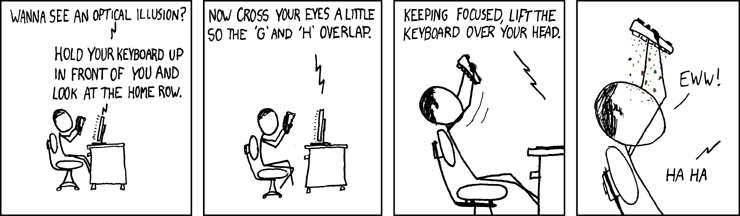
\includegraphics[width=\textwidth]{../common/images/keyboards_are_disgusting}
%     \imagesource{https://xkcd.com/237/}
%     \vfill
% \end{frame}
%
\frame[plain]{
    \titlepage

    \notes{
        \item welcome the audience
        \item introduce ourselves
        \item explain this is our bachelor's thesis defense
    }
}

\begin{frame}{\contentsname}
    \iffinal
        \tableofcontents[subsectionstyle=hide,subsubsectionstyle=hide]
    \else{
        \begin{multicols*}{2}
            \tableofcontents[subsubsectionstyle=hide]
            \vfill\null
        \end{multicols*}
    }\fi

    \notes{
        \item 1, 2 Paul
        \item 3, 4 Caro
        \item Demo \& Conclusion together
    }
\end{frame}

\AtBeginSection[]{
    \begin{frame}{\insertsectionhead}
        \tableofcontents[
            currentsection,
            currentsubsection,
            subsectionstyle=show/show/hide,
            subsubsectionstyle=hide,
        ]
    \end{frame}

    \addtocounter{framenumber}{-1}% If you don't want them to affect the slide number
}

\section{Introduction}

\subsection{Motivation}
\begin{frame}{Motivation}{Traditional Keyboards}
    \begin{columns}[T]
        \begin{column}{0.5\textwidth}
            \only<1->{
                \textbf{Pros}
                \begin{itemize}
                    \item easy to learn
                    \item precise
                    \item universal
                    \item cheap
                \end{itemize}
            }
        \end{column}
        \begin{column}{0.5\textwidth}
            \only<2->{
                \textbf{Cons}
                \begin{itemize}
                    \item poor ergonomics
                    \item depends on motor abilities
                    \item not adjustable to task $\rightarrow$ ,,shortcuts''
                \end{itemize}
            }
        \end{column}
    \end{columns}
    \vspace{2em}
    \begin{columns}[T]
        \begin{column}{0.5\textwidth}
            \only<4->{
                \textbf{Alternatives}
                \begin{itemize}
                    \item voice recognition
                    \item handwriting recognition
                    \item visual methods (eye tracking)
                \end{itemize}
            }
        \end{column}
        \begin{column}{0.5\textwidth}
            \only<3->{
                \centering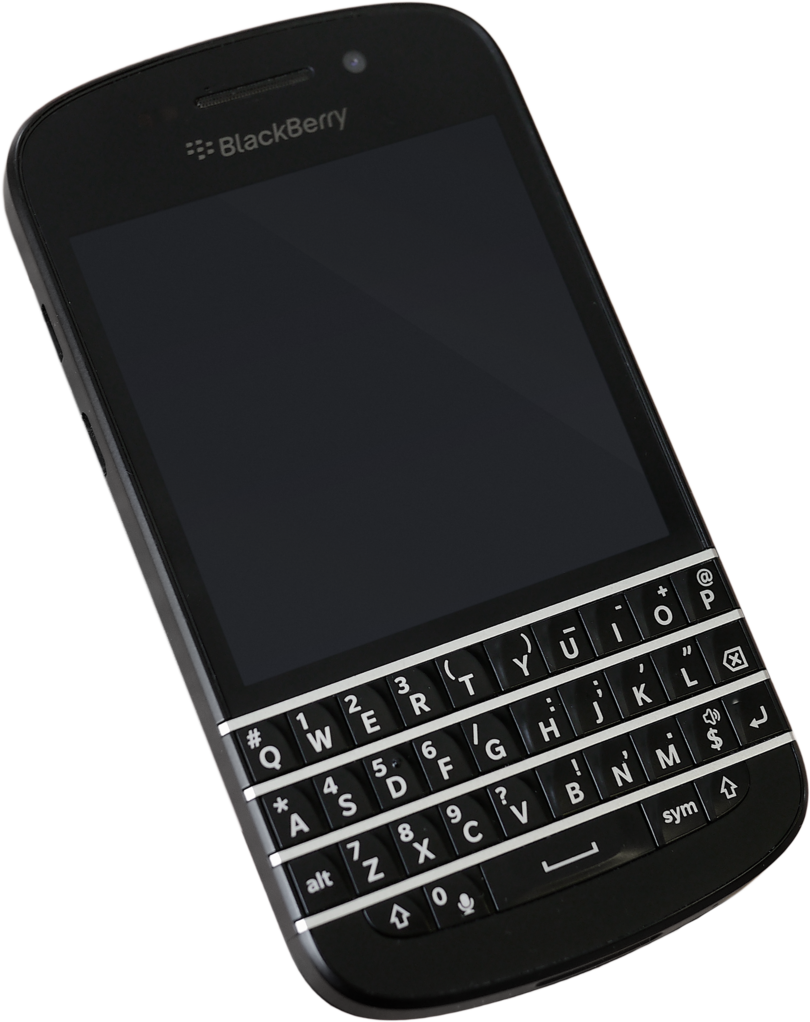
\includegraphics[width=0.4\textwidth]{../common/images/blackberry}
            }
        \end{column}
    \end{columns}

    \only<3->{
        \flushright
        \imagesource{https://en.wikipedia.org/wiki/File:Blackberry-Q10-transparent.png}
    }

    \notes {
        \item present pros and cons
        \item it's still the most common choice
        \item phones get smaller $\rightarrow$ deviceless
        \item \textbf{voice}: inaccurate, only nat. language, environment dependent
        \item \textbf{handwriting}: slow, touch screen, surface, inaccurate
        \item \textbf{visual methods}: very slow, good for handicapped users
    }
\end{frame}

\subsection{Vision}
\begin{frame}{Vision}
    \begin{enumerate}
        \item<1-> record finger movements and input while typing
        \item<2-> use machine learning for input prediction
        \item<3-> remove keyboard
        \item<4-> type everywhere
    \end{enumerate}

    \notes{
        \item simple to generate learning data
        \item complex movement we don't fully predict: (example with B key)
        \item \textbf{BUT FIRST!} let's see who did this already
    }
\end{frame}

\subsection{Related Work}
\begin{frame}{Related Work}{Sensor Gloves}
    \begin{itemize}
        \item gesture detection \citep{web:cyberglove} \citep{zimmerman-flex-gloves} \citep{imu-emg}
        \item sign language detection \citep{imu-emg} \cite{mehdi-sign-language-glove}
        \item music generation \citep{web:mimugloves}
        \item medical applications \citep{cavallo-senshand-parkinsons}
    \end{itemize}

    $\rightarrow$ overview at \citetitle{web:mimugloves-overview} \citep{web:mimugloves-overview}

    \notes{
        \item flex sensor gloves started 1987
    }
\end{frame}

\begin{frame}{Related Work}{Alternative Keyboard Inputs}
    \begin{itemize}
        \item buttons on glove \citep{web:keyglove}
        \item braille gloves \citep{braille-gloves}
        \item \citetitle{ellithorpe-kinect-typing} \citep{ellithorpe-kinect-typing} $\rightarrow$ Kinect
    \end{itemize}

    \centering
    \begin{figure}
        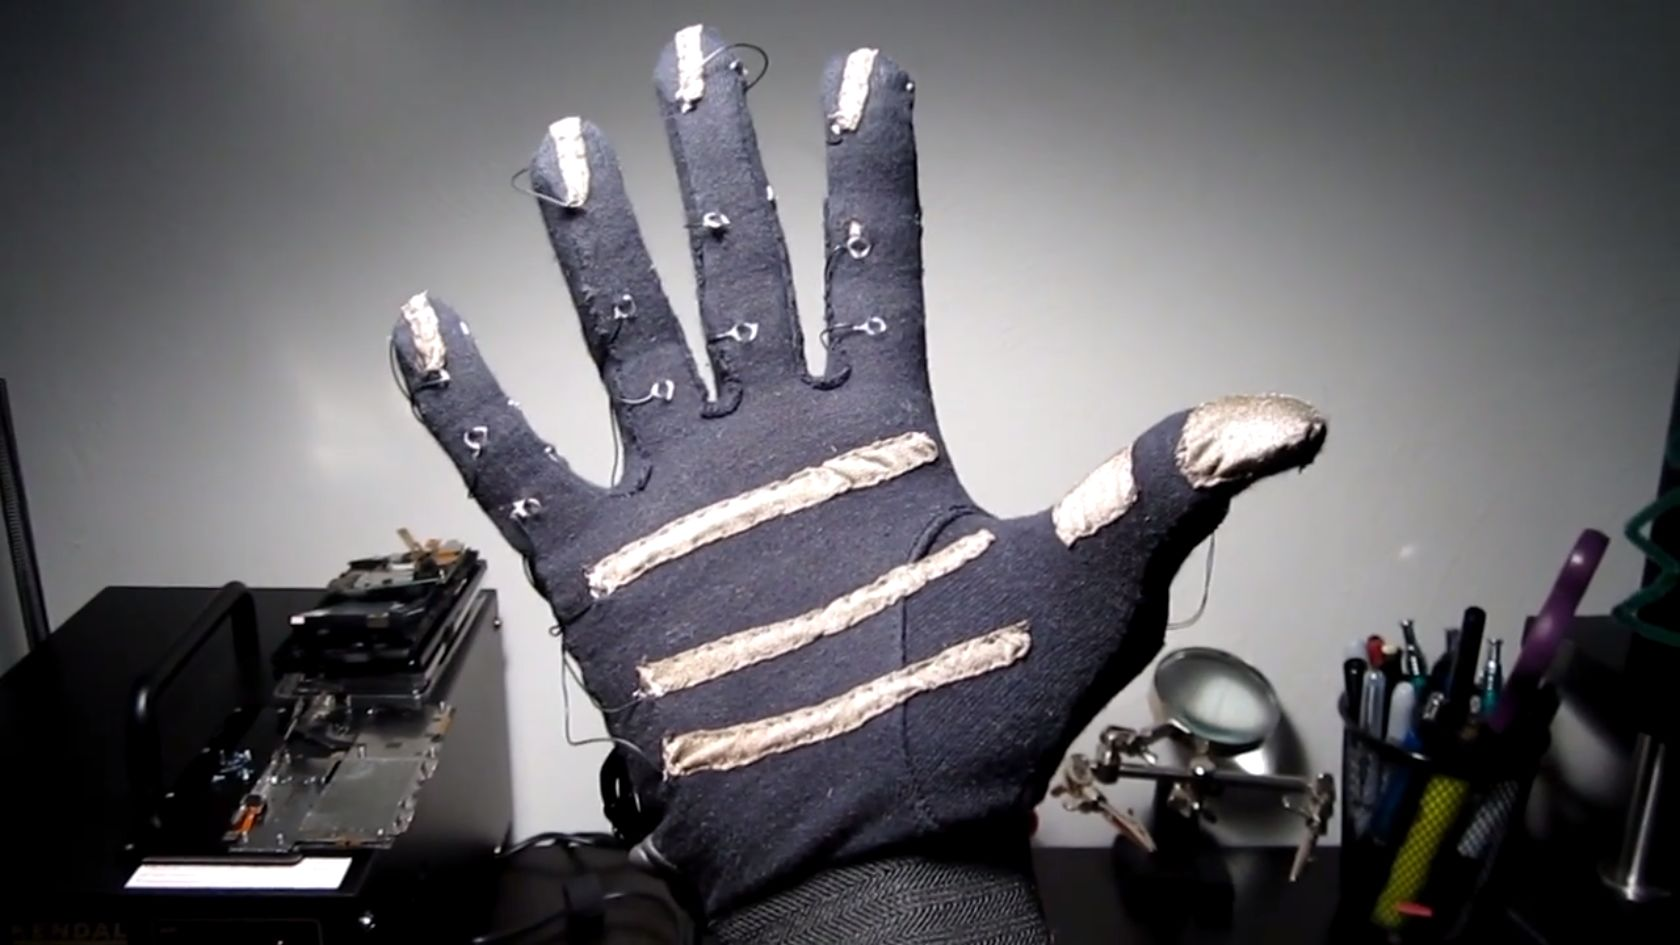
\includegraphics[width=0.55\textwidth]{../common/images/keyglove}
        \caption{The Keyglove - a wearable, wireless, open-source input device}
    \end{figure}
    \imagesource{https://vimeo.com/23269969}
\end{frame}

\begin{frame}{Related Work}{Commercial Products}
    \begin{itemize}
        \item \citetitle{web:gest} \citep{web:gest} {\scriptsize($\text{\$ }199,988$ on Kickstarter)}
        \item \citetitle{web:senseboard} \citep{web:senseboard}
        \item \citetitle{web:hi5vrglove} \citep{web:hi5vrglove} $\rightarrow$ VR Gaming
    \end{itemize}
    \begin{columns}[T]
        \begin{column}{0.48\textwidth}
            \begin{figure}
                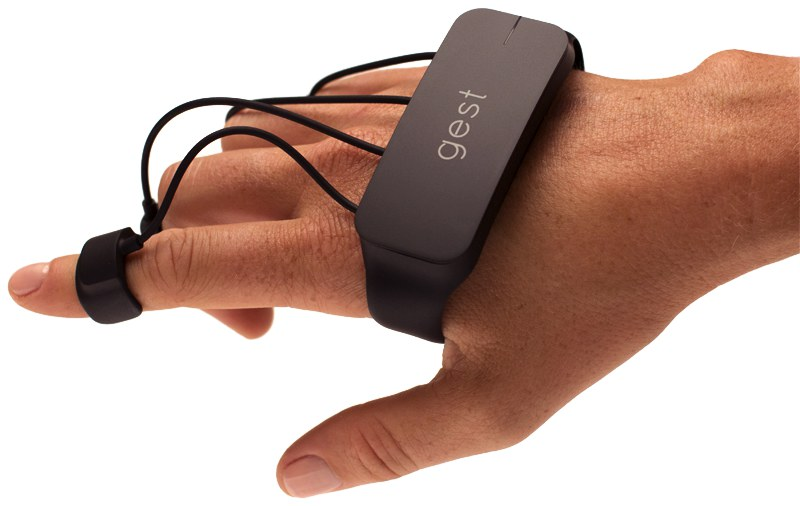
\includegraphics[height=3cm]{../common/images/gest}
                \imagesource{https://gest.co/}
                \caption{Gest general purpose interaction wearable}
            \end{figure}
        \end{column}
        \begin{column}{0.48\textwidth}
            \begin{figure}
                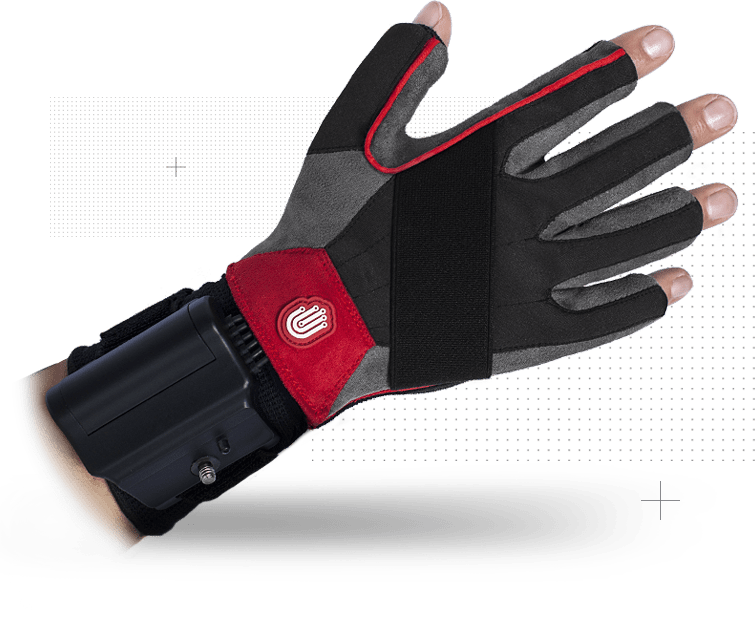
\includegraphics[height=3cm]{../common/images/hi5vr-glove}
                \imagesource{http://hi5vrglove.com/}
                \caption{Noitom Hi5 VR Glove}
            \end{figure}
        \end{column}
    \end{columns}

    \notes{
        \item \textbf{gest}
        \item raised \textasciitilde 200k USD on kickstarter in Oct 2015
        \item out of business within half a year, no funding
        \item \textbf{senseboard}
        \item weird project, no information available, no images
        \item same idea as we did
        \item \textbf{hi5vrglove}
        \item intended for VR gaming
        \item very new
        \item no typing software
        \item same hardware specs
        \item \textbf{gest at least advertised with keyboard functionality}
    }
\end{frame}

\begin{frame}{Related Work}{In Research}
    \center
    \vfill
    no research project combines\\[1em]
    sensor + keyboard data $\rightarrow$ machine learning
    \vfill
\end{frame}

\subsection{Project Goal}
\begin{frame}{Project Goal}
    Of course we won't build a fully working keyboard in 2 bachelor theses.
    \pause
    \vspace{2em}
    \begin{block}{Goal}
        Design a system for recording characteristic hand movements of typing
        and the corresponding input.\\[1em]

        Define an approach for utilizing machine learning to map the recorded
        data back to the keyboard input.\\[1em]

        Evaluate the quality of such mapping and discuss whether this principle
        could be turned into a working keyboard alternative.
    \end{block}
\end{frame}

\section{System design}

\subsection{Desired System Properties}

\begin{frame}{Desired System Properties}
    \begin{itemize}
        \item utilizes machine learning
        \item detects characteristic values
            \begin{itemize}
                \item fast (goal 100Hz)
                \item accurate
                \item independent of pose
            \end{itemize}
        \item non-obstructive
            \begin{itemize}
                \item flexible
                \item wireless
                \item light
            \end{itemize}
        \item software suitable for fast prototyping
        \item cheap
    \end{itemize}
\end{frame}

\subsection{Sensors}

\begin{frame}{Sensors}{Possible Choices}
    \begin{figure}
        \centering
        \begin{columns}[t]
            \column{.3\textwidth}
            \textbf{Flex sensors}
            \begin{minipage}[t][\textwidth][c]{\textwidth}
                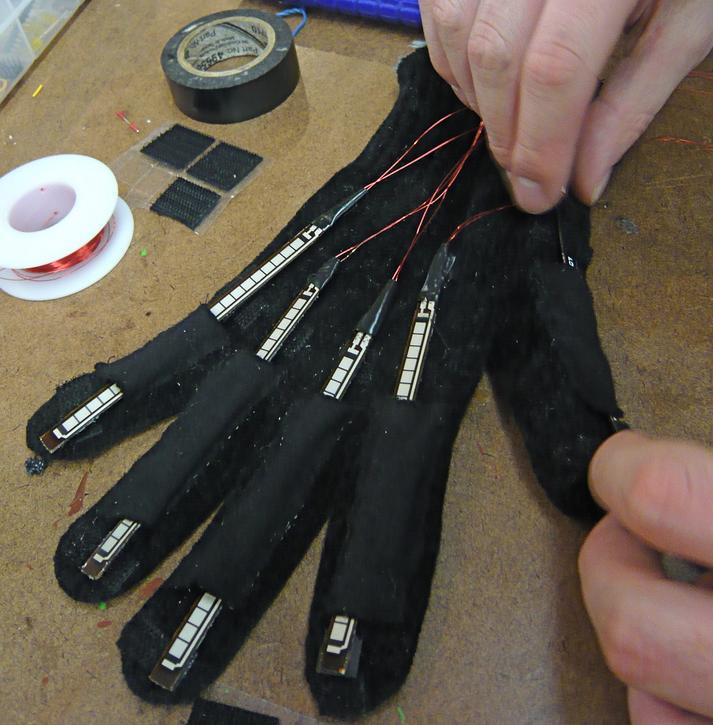
\includegraphics[width=\textwidth]{../common/images/flex-glove}
            \end{minipage}
            \imagesource{https://www.flickr.com/photos/indiamos/3060497602}

            \uncover<2->{
                \column{.3\textwidth}
                \textbf{Visual system}
                \begin{minipage}[t][\textwidth][c]{\textwidth}
                    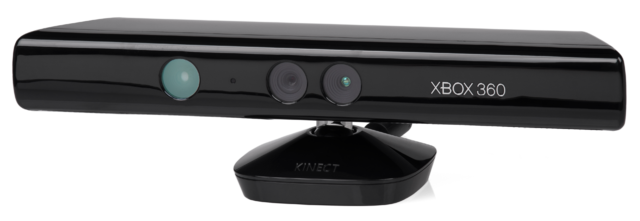
\includegraphics[width=\textwidth]{../common/images/kinect}
                \end{minipage}
                \imagesource{https://de.wikipedia.org/wiki/Kinect\#/media/File:Xbox-360-Kinect-Standalone.png}
            }

            \uncover<3->{
                \column{.3\textwidth}
                \textbf{IMUs}
                \begin{minipage}[t][\textwidth][c]{\textwidth}
                    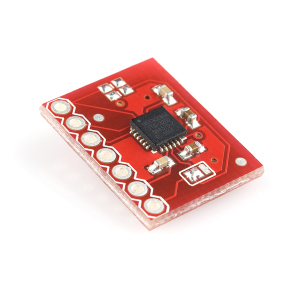
\includegraphics[width=\textwidth]{../common/images/mpu-9150}
                \end{minipage}
                \imagesource{https://organicmonkeymotion.wordpress.com/category/propeller/}
            }
        \end{columns}
        \caption{Possible types of sensors; \emph{left} resistive flex sensors\uncover<2->{, \emph{center} Kinect for Xbox 360}\uncover<3->{, \emph{right}
        InvenSense MPU-9150 IMU}}
    \end{figure}

    \notes{
        \item flex sensors
            \begin{itemize}
                \item only 1 dimensional
                \item not suited for horizontal movement
                \item only relative data
            \end{itemize}
        \item Visual system
            \begin{itemize}
                \item hard to extract characteristic data
                \item often inaccurate
                \item no freedom gain
            \end{itemize}
        \item IMUs
            \begin{itemize}
                \item small, cheap, robust
                \item easy to use and understand
                \item provide good accuracy high dimensional data
                \item capture characteristic movement (ie. yaw AND pitch)
            \end{itemize}
        \item \textbf{\large{}6 IMUS, 5 fingers, 1 for reference at back of hand}
    }
\end{frame}

\begin{frame}<1>[label=imus]{Sensors}{Inertial Measurement Units (IMUs)}
    \small
    % \begin{tabular}{llll}
    %     \raisebox{-4mm}{
\includegraphics[width=1cm,height=1cm]{../common/images/icon-accel}} &
    %     \textbf{Accelerometer} & 3 DoF & linear acceleration (and gravity) \\[1em]
    %     \raisebox{-4mm}{
\includegraphics[width=1cm,height=1cm]{../common/images/icon-gyro}} &
    %     \textbf{Gyroscope} & 3 DoF & angular velocity \\[1em]
    %     \raisebox{-4mm}{
\includegraphics[width=1cm,height=1cm]{../common/images/icon-magnet}} &
    %     \textbf{Magnetometer} & 3 DoF & compass, absolute reference
    % \end{tabular}
    %
    \begin{figure}
        \begin{tikzpicture}[
            icon/.style={
                inner sep=0pt,
            },
            icontext/.style={
                text width=3cm,
                align=center,
                font=\scriptsize,
            },
        ]
            \node[icon] (gyro) at (0, 0)
                {
\includegraphics[width=1cm,height=1cm]{../common/images/icon-gyro}};
            \node[icon,left=3cm of gyro] (accel)
                {
\includegraphics[width=1cm,height=1cm]{../common/images/icon-accel}};
            \node[icon,right=3cm of gyro] (magnet)
                {
\includegraphics[width=1cm,height=1cm]{../common/images/icon-magnet}};

            \node[icontext,above=1mm of accel] (acceltext) {\textbf{Accelerometer}};
            \node[icontext,above=1mm of gyro] (gyrotext) {\textbf{Gyroscope}};
            \node[icontext,above=1mm of magnet] (magnettext) {\textbf{Magnetometer}};

            \only<1> {
                \node[flowchart node,below=6mm of gyro] (fusion) {Sensor Fusion};
            }
            \only<2> {
                \node[flowchart node,below=6mm of gyro] (fusion) {``BSX3.0 FusionLib''\\software};
            }

            \node[flowchart node,below=4mm of fusion] (quat) {Quaternion};

            \draw[flowchart arrow]  (accel.south) |- (fusion.west);
            \draw[flowchart arrow]  (gyro) -- (fusion.north);
            \draw[flowchart arrow]  (magnet) |- (fusion.east);

            \draw[flowchart arrow]  (fusion) -- (quat);

            \uncover<2-> {
                \node[icontext,above=0pt of acceltext] {14 bit\\$\pm{}2..16g$\\$10^{-3}g/LSB$};
                \node[icontext,above=0pt of gyrotext] {16 bit\\$\pm{}125..2000^{\circ}s^{-1}$};
                \node[icontext,above=0pt of magnettext] {heading $\pm{}2.5^{\circ}$};
            }
        \end{tikzpicture}
       \label{fig:sensor_fusion}
       \caption{Sensor Fusion Overview}
    \end{figure}
\end{frame}

\begin{frame}{Sensors}{Wearable BNO055 Nano Board}
    \begin{columns}[T]
        \begin{column}{0.4\textwidth}
            \uncover<1->{
                \begin{figure}
                    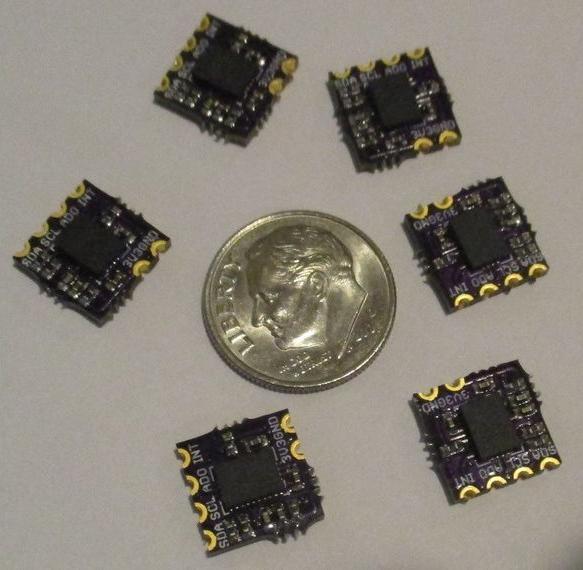
\includegraphics[width=\textwidth]{../common/images/bno055-nano-boards}
                    \imagesource{https://www.tindie.com/products/onehorse/wearable-bno055-nano-board/}
                    \caption{Wearable BNO055 Nano Board}
                \end{figure}
            }
        \end{column}
        \begin{column}{0.6\textwidth}
            \uncover<2->{
                \begin{itemize}
                    \item 32 bit System-in-Package
                    \item tiny ($\SI{10}{mm} \times \SI{10}{mm}$)
                    \item easy to use
                    \item good performance (\textasciitilde{}\SI{100}{Hz})
                \end{itemize}
            }

            \uncover<3->{
                however...
                \begin{itemize}
                    \item ca. \EUR{24} each
                    \item ships from USA
                    \item gyro clipping problems
                \end{itemize}
            }
        \end{column}
    \end{columns}

    \vfill

    \notes{
        \item we had to choose between MPU-9150 and BNO-055
        \item both seemed fit
        \item BNO easier to use
        \item very small board available
        \item but more expensive
    }

    % \footnotetext[1]{\tiny{}\url{https://ae-bst.resource.bosch.com/media/_tech
    % /media/product_flyer/BNO055_Productflyer_BST_20170109.pdf}}
    % https://ae-bst.resource.bosch.com/media/_tech/media/datasheets/BST_BNO055_DS000_14.pdf
\end{frame}

\againframe<1-2>{imus}


\subsection{Microprocessor}

\begin{frame}{Microprocessor}{Adafruit Feather M0 WiFi}
    \begin{columns}[T]
        \begin{column}{0.5\textwidth}
            \uncover<2->{
                \begin{itemize}
                    \item very small and lightweight (6.1g)
                    \item on-board WiFi
                    \item 6 SERCOMs (SPI/I2C/UART)
                \end{itemize}
            }
            \uncover<3->{
                \begin{itemize}
                    \item Arduino\textsuperscript{\textregistered} compatible
                    \item 256KB FLASH, 32KB SRAM
                    \item LiPo charger
                \end{itemize}
            }
            \uncover<4->{
                however...
                \begin{itemize}
                    \item no EEPROM
                    \item ca. \EUR{40} each
                \end{itemize}
            }
        \end{column}

        \begin{column}{0.5\textwidth}
            \uncover<1->{
                \begin{figure}
                    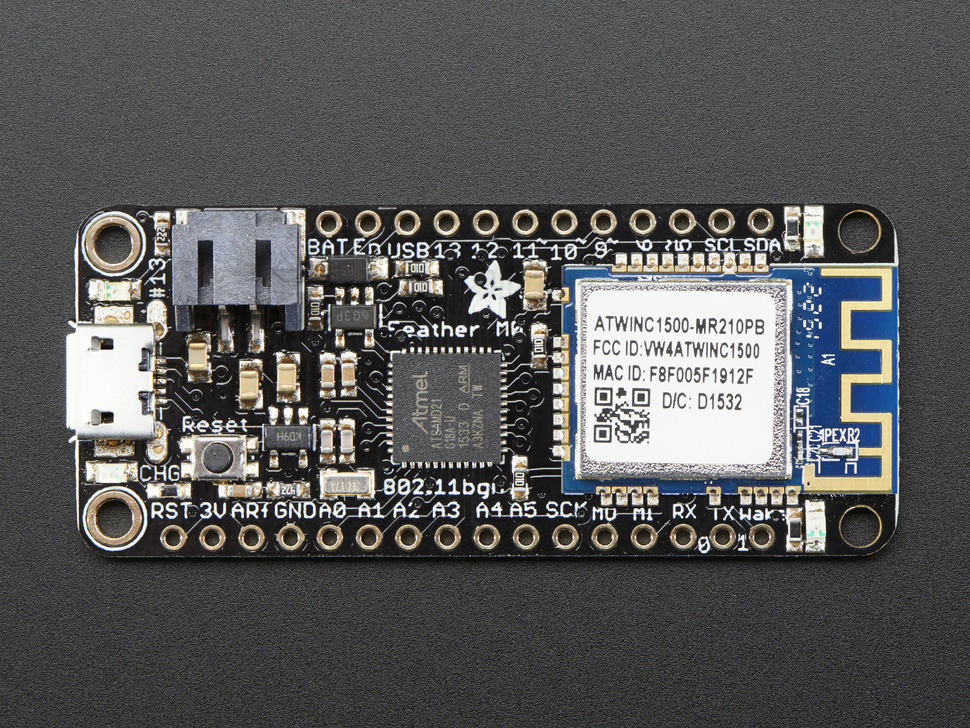
\includegraphics[width=\textwidth]{../common/images/feather-m0-wifi}
                    \imagesource{https://www.adafruit.com/product/3010}
                    \caption{Adafruit Feather M0 WiFi - ATSAMD21 + ATWINC1500 product image}
                \end{figure}
            }
        \end{column}
    \end{columns}

    \notes{
        \item we chose this microprocessor
        \item alternative was Teensy 3.2, but that had some disadvantages
        \item small \& light $\rightarrow$ required for hand-attached device
        \item WiFi $\rightarrow$ no cable that impedes movement
        \item enough SERCOMs
        \item LiPo charger is useful
        \vspace{1em}
        \item we need EEPROM for WiFi credentials $\rightarrow$ so we attached one ourselves
        \item more expensive than Teensy
    }
\end{frame}

\subsection{Architecture}

\begin{frame}<1-2>[label=overview]
    \frametitle<1-2>{Architecture}
    \frametitle<3>{Glove $\leftrightarrow$ PC connection}
    \frametitle<4->{Machine Learning}

    \scalebox{0.7}{
        \begin{tikzpicture}[
    onslide/.code args={<#1>#2}{%
        \ifdefined\only
        \only<#1>{\pgfkeysalso{#2}}%
        \else
        #2
        \fi
    },
    every node/.style={
        font=\small,
        inner sep=0pt,
        thick,
    },
    node distance=2cm,
    database/.style={
        cylinder,
        shape border rotate=90,
        aspect=0.2,
        draw,
        minimum width=2.5cm,
        text width=2.5cm,
        align=center,
        minimum height=1.5cm,
    },
    node/.style={
        rectangle,
        draw,
        text width=2.5cm,
        align=center,
        minimum height=1cm,
        rounded corners=2pt,
    },
    arrow/.style={
        thick,
        ->,
        >=stealth,
    },
    learning/.style={
        dashed,
    },
    applying/.style={
        very thick,
    },
    radiation/.style={
        decorate,
        decoration={expanding waves,angle=10,segment length=4pt}
    },
    wire/.style={
        % draw=gray,
    },
    sensor/.style={
        node,
        minimum width=5mm,
        minimum height=5mm,
        text width=0,
        draw,
        rectangle,
        rounded corners=0,
    },
    highlight/.style={
        draw=primary,
        color=primary,
        fill=primary!10!white,
    },
    drawhighlight/.style={
        thick,
        draw=primary,
    },
    texthighlight/.style={
        color=primary,
    },
]

    \coordinate (legend) at (6.5, 0.2);
    \draw[thick,wire]           ($ (legend) + (0,    0) $) -- node[at end, right, xshift=0.2cm] {Wire}  ++(0.5, 0);
    \draw[thick,arrow,learning] ($ (legend) + (0, -0.6) $) -- node[at end, right, xshift=0.2cm] {Learn} ++(0.5, 0);
    \draw[thick,arrow,applying] ($ (legend) + (0, -1.2) $) -- node[at end, right, xshift=0.2cm] {Apply} ++(0.5, 0);
    \draw ($ (legend) + (-0.2, 0.3) $) rectangle ++(2, -1.8);

    \node[node]
        (serialparser)
        at (0, 0)
        {Serial Parser};

    \node[node,left=2cm of serialparser]
        (sender)
        {Micro-\\processor};

    \node[sensor,below left=7mm and 0.5cm of sender.south]  (sensor1) {};
    \node[sensor,below=2mm of sensor1] (sensor2) {};
    \node[sensor,below=2mm of sensor2] (sensor3) {};
    \node[sensor,below right=7mm and 0.5cm of sender.south] (sensor4) {};
    \node[sensor,below=2mm of sensor4] (sensor5) {};
    \node[sensor,below=2mm of sensor5] (sensor6) {};

    \node[below=3cm of sender] {Sensors};
    \draw[wire,onslide={<2> drawhighlight}] (sensor1) -| ($ (sender.south) + (-0.2, 0) $);
    \draw[wire,onslide={<2> drawhighlight}] (sensor2) -| ($ (sender.south) + (-0.12, 0) $);
    \draw[wire,onslide={<2> drawhighlight}] (sensor3) -| ($ (sender.south) + (-0.04, 0) $);
    \draw[wire,onslide={<2> drawhighlight}] (sensor4) -| ($ (sender.south) + (0.2, 0) $);
    \draw[wire,onslide={<2> drawhighlight}] (sensor5) -| ($ (sender.south) + (0.12, 0) $);
    \draw[wire,onslide={<2> drawhighlight}] (sensor6) -| ($ (sender.south) + (0.04, 0) $);

    \draw[radiation,onslide={<3> drawhighlight}]
        ([xshift=2mm,yshift=-0.3cm]sender.east) -- node[midway,yshift=-0.6cm,onslide={<3> texthighlight}] {or WiFi} ([xshift=-2mm,yshift=-0.3cm]serialparser.west);

    \draw[very thick,wire,onslide={<3> drawhighlight}]
        ([yshift=0.2cm]sender.east) -- node[midway,yshift=0.3cm,onslide={<3> texthighlight}] {USB} ([yshift=0.2cm]serialparser.west);

    \node[node,right=1cm of serialparser]
        (keyboard)
        {Keyboard\\Listener};

    \node[database]
        (bag)
        at ($ (serialparser) + (1.75, -2) $)
        {ROS Bag};

    \node[node,text width=6cm,onslide={<5> highlight}]
        (preprocessing)
        at ($ (serialparser) + (1.75, -4) $)
        {Preprocessing};

    \node[node, below=1cm of preprocessing.south west,anchor=north west,onslide={<5> highlight}]
        (apply)
        {Apply\\Network};

    \node[database, below=1.5cm of preprocessing.south east,anchor=east,onslide={<5> highlight}]
        (model)
        {Saved Model};

    \node[node, right=1cm of preprocessing,onslide={<5> highlight}]
        (sampling)
        {Sampling};

    \node[node, below=1cm of sampling,onslide={<5> highlight}]
        (learning)
        {Learning};

    \node[node, text width=9.5cm]
        (os)
        at ($ (apply) + (3.5, -2) $)
        {Operating System};

    \draw [arrow,applying] ($ (serialparser) + (-0.5,-0.5) $) -- +(0, -3);
    \draw [arrow,learning] ($ (serialparser) + (0,-0.5) $) -- +(0, -1) -- (bag);
    \draw [arrow,learning] ($ (keyboard) + (0,-0.5) $) -- +(0, -1) -- (bag);
    \draw [arrow,learning] (bag) -- (preprocessing);
    \draw [arrow,applying] ($ (preprocessing) + (-2.25,-0.5) $) -- +(0, -1);
    \draw [arrow,applying] (model) -- (apply);
    \draw [arrow,learning] (preprocessing) -- (sampling);
    \draw [arrow,learning] (sampling) -- (learning);
    \draw [arrow,learning] (learning) -- (model);
    \draw [arrow,applying] ($ (apply) + (-0.5,-0.5) $) -- +(0, -1);

    \draw[dotted,line width=2pt] ($ (serialparser) !.5! (sender) + (0, -1.5) $) -- node[at end] (bottom) {} +(0, -8);
    \draw[dotted,line width=2pt] ($ (serialparser) !.5! (sender) + (0, 1) $) -- +(0, 0.5);

    \node[anchor=north west,right=10mm of bottom,yshift=0.5em] {\large{}\textbf{HOST PC}};
    \node[anchor=north east,left=10mm of bottom,yshift=0.5em] {\large{}\textbf{GLOVE}};

    \ifdefined\setbeamertemplate
        \only<1-4>{
            \node[node, anchor=north west, minimum width=9.6cm, minimum height=3.2cm, fill=white] at (preprocessing.north west) {Machine learning};
        }
    \fi
\end{tikzpicture}

    }
\end{frame}

\begin{frame}<1-4>{I2C Bus}{Requirements}
    $$\frac{6\text{ IMUs}}{2\;\frac{\text{addresses}}{\text{IMU}}} = 3\text{ buses}$$

    \pause
    \vspace{1em}

    \begin{table}
    \begin{tabular}{|r||c|c|c|c||c|c|c|c||l|}
        \hline
        & \multicolumn{4}{c||}{Primary pads} & \multicolumn{4}{c|}{Alternative pads} & \\ \hline
        SERCOM
            & 0 & 1 & \color{lightgray}2 & \color{lightgray}3
            & 0 & 1 & \color{lightgray}2 & \color{lightgray}3 & Used by \\ \hline
        0
            & \only<2>{4}
            & 3
            & \color{lightgray}1
            & \color{lightgray}0
            & \only<4>{\cellcolor{primary!25}}A3
            & \only<4>{\cellcolor{primary!25}}A4
            & \color{lightgray}\only<2>{8}
            & \color{lightgray}9
            & Serial1 \\
        1
            & 11
            & 13
            & \color{lightgray}10
            & \color{lightgray}12
            &
            &
            &
            &
            & \\
        2
            & 22
            &
            & \color{lightgray}\only<2>{2}
            & \color{lightgray}5
            & \only<2>{4}
            & 3
            & \color{lightgray}1
            & \color{lightgray}0
            & \\
        3
            & 20
            & 21
            & \color{lightgray}6*
            & \color{lightgray}\only<2>{7*}
            & \only<4>{\cellcolor{primary!25}}11
            & \only<4>{\cellcolor{primary!25}}13
            & \color{lightgray}10
            & \color{lightgray}12
            & Default I2C \\
        4
            & 22
            &
            & \color{lightgray}23*
            & \color{lightgray}24*
            & A1
            & A2
            & \color{lightgray}\only<2>{2}
            & \color{lightgray}5
            & SPI \\
        5
            & A5*
            &
            & \color{lightgray}6
            & \color{lightgray}\only<2>{7}
            & \only<4>{\cellcolor{primary!25}}20
            & \only<4>{\cellcolor{primary!25}}21
            &
            &
            & Debug Port\\
        \hline
    \end{tabular}
    \vspace{2mm}
    {\scriptsize* need to be configured as \emph{SERCOM alt}}
    \caption{Available SERCOM pin pads on Adafruit Feather M0 WiFi}
    \end{table}

    \notes {
        \item these are the available pins for the different SERCOMs on the Feather M0
        \item we need pads 0 und 1 for I2C (fixed)
        \item pins 2, 4, 7, 8 are required for WiFi
        \item so we picked the \textcolor{red}{red marked}
    }
\end{frame}

\begin{frame}[fragile]{I2C Bus}{Arduino Setup}
    \begin{minted}[style=arduino,fontsize=\scriptsize]{c}
#include <Wire.h>
#include <wiring_private.h>

TwoWire wire0(&sercom0, A3, A4);
TwoWire wire1(&sercom3, 11, 13);
TwoWire wire2(&sercom5, 20, 21);

void setup() {
    wire0.begin(); wire0.setClock(400000L);
    wire1.begin(); wire1.setClock(400000L);
    wire2.begin(); wire2.setClock(400000L);
    delay(100);

    pinPeripheral(A3, PIO_SERCOM_ALT); // SERCOM0.0 (alt)
    pinPeripheral(A4, PIO_SERCOM_ALT); // SERCOM0.1 (alt)
    pinPeripheral(11, PIO_SERCOM_ALT); // SERCOM3.0 (alt)
    pinPeripheral(13, PIO_SERCOM_ALT); // SERCOM3.1 (alt)
    pinPeripheral(20, PIO_SERCOM_ALT); // SERCOM5.0 (alt)
    pinPeripheral(21, PIO_SERCOM_ALT); // SERCOM5.1 (alt)
}
    \end{minted}
\end{frame}

\againframe<3>{overview}

\begin{frame}[fragile]{Glove $\leftrightarrow$ PC Connection}{WiFi}
    \begin{columns}[T]
        \begin{column}{0.5\textwidth}
            \begin{minted}[style=arduino,fontsize=\tiny]{c}
// Setup
WiFi.setPins(8, 7, 4, 2);
WiFi.begin();

// Scan for networks (optional)
uint8_t ssidCount = WiFi.scanNetworks();
for (uint8_t i = 0; i < ssidCount; i++) {
    printf("- %s\n", WiFi.SSID(i));
}

// Connect to WPA2 network
uint8_t status = WiFi.begin(MY_SSID, MY_PASSPHRASE);
while (status != WL_CONNECTED) {
    delay(500);
    status = WiFi.status();
}

// Send data via UDP
WiFiUDP wifiUdp;
wifiUdp.begin(8080);
wifiUdp.beginPacket(TARGET_IP, TARGET_PORT);
wifiUdp.write(buffer, length);
wifiUdp.endPacket();
            \end{minted}
        \end{column}
        \begin{column}{0.5\textwidth}
            Capabilities
            \begin{itemize}
                \item WEP \& WPA2
                \item Scan networks
                \item UDP, TCP, SSL
                \item HTTP Client
                \item HTTP Server
            \end{itemize}
        \end{column}
    \end{columns}
\end{frame}


\begin{frame}{System design}{Other Considerations}
    \begin{itemize}
        \item serial protocol for data transmission
        \item attachment to the hand
        \item use ROS for recording \& data analysis
    \end{itemize}
\end{frame}
%
% \subsection{Data Transmission}

% \setbeamercovered{transparent}
% \begin{frame}{Data Transmission}{Protocol Requirements}
%     \centering
%     \vfill\null
%     \def\arraystretch{1.5}
%     \scriptsize
%     \begin{tabular}{p{0.45\textwidth}|p{0.45\textwidth}}
%         \textbf{Requirement} & \textbf{Means} \\ \hline\hline
%         fast $\rightarrow$ lightweight & self made solution \pause \\
%         supports USB \& WiFi & package based protocol \pause \\
%         simple to write \& parse & simple buffer layout \pause \\
%         robust & package start/end checks \pause \\
%         flexible & versioned \pause \\
%         time critical & timestamps included in every message \pause \\
%         metadata: imu count, sensibility & header packet
%     \end{tabular}
%     \vfill\null
% \end{frame}
% \setbeamercovered{invisible}


\section{Machine Learning}

\subsection{Introduction}

\againframe<4-5>{overview}
%TODO: more machine learning examples (decision tree, ....)
%TODO: neuronal nets erklären

%TODO: RNN new graphic

\begin{frame}{Introduction}{Supervised and Unsupervised learning}
    \begin{table}
        \def\arraystretch{1.5}
        \scriptsize
        \begin{tabular}{r | p{.3\textwidth} | p{.3\textwidth}}
            & Supervised & Unsupervised \\
            \hline
            Learning Data & \tabitem input X &  \tabitem input X\\
            & \tabitem target values Y & \\
            What is learned & mapping function $Y \approx f(X)$ & model of data structure\\
            Examples & \tabitem classification & \tabitem clustering \\
            & \tabitem regression & \tabitem association \\
        \end{tabular}
    \end{table}

    \notes{
        \item warum machine learning (und nicht vorgegebene gesten erkennen)
        \item supervised unsupervised
        \item vorteile/ nachteile
        \item warum supervised
    }
\end{frame}

\subsection{Neural Networks}
\begin{frame}{Neural Networks}{Strengths and Weaknesses \cite{tu-advantages-disadvantages-neural-networks}}
    \begin{columns}
        \begin{column}{0.5\textwidth}
            \textbf{Pros}
            \begin{itemize}
                \item general-purpose
                \item many variations
                \item fast to apply once learned
                \item able to detect complex relationships
            \end{itemize}
        \end{column}
        \begin{column}{0.5\textwidth}
            \textbf{Cons}
            \begin{itemize}
                \item requires large dataset
                \item blackbox\footnotemark[1], difficult to ``understand''
                \item slow to learn
                \item can overfit
            \end{itemize}
        \end{column}
    \end{columns}

    \footnotetext[1]{there are some rule-extraction algorithms \cite{web:misconceptions-neural-network}}


    \notes{
        \item \textbf{ARE }general-purpose
        \item easiliy generate data
        \item not important how (we dont know movement of fingers)
        \item tradeoff: complex calculation <-> data needed to learn
        \item bridge: NN we were interested in
    }
\end{frame}

\subsection{Recurrent Neural Networks}
\begin{frame}{Recurrent Neural Networks}
    \centering
    \vfill
    \begin{figure}
        \begin{tikzpicture}[
    ->,
    >=stealth',
    shorten >=1pt,
    auto,
    node distance=2.2cm,
    semithick,
    layer/.style={
        draw,
        minimum width=0.9cm,
        minimum height=6cm,
    },
    bend angle=15,
    every state/.style={
        very thick,
        fill=white,
        distance=1.2,
        minimum size=0.5cm,
    },
]
    \node[state]         (D)  {};
    \node[state]         (A) [above left=1cm and 2.2cm of D] {};
    \node[state]         (B) [below left=1cm and  2.2cm of D] {};

    \node[state]         (C) [above of=D] {};

    \node[state]         (E) [below of=D] {};
    \node[state]         (F) [right =2.2cm of D] {};

    \path   (A) edge              node {} (C)
                edge              node {} (D)
                edge              node {} (E)

              (B) edge              node {} (C)
                edge              node {} (D)
                edge              node {} (E)

            (C) edge [loop above,gray] node {} (C)
                edge              node {} (F)
                edge [bend left,gray]  node {} (D)
                edge [bend left,gray]  node {} (E)

            (D) edge [loop above,gray] node {} (D)
                edge              node {} (F)
                edge [bend left,gray]  node {} (C)
                edge [bend left,gray]  node {} (E)

            (E) edge [loop above,gray] node {} (E)
                edge [bend left,gray]  node {} (C)
                edge [bend left,gray]  node {} (D)
                edge              node {} (F);


    \node[layer,label=below:{\small\textbf{input}}] at ($(A) !.5! (B)$) {};
    \node[layer,label=below:{\small\textbf{hidden}}] at (D) {};
    \node[layer,label=below:{\small\textbf{output}}] at (F) {};
    % \draw ($(E.south west) - (0.2, 0.2)$) rectangle ($(C.north east) + (0.2, 0.2)$);
    % \draw ($(F.south west) - (0.2, 0.2)$) rectangle ($(F.north east) + (0.2, 0.2)$);

\end{tikzpicture}

        \caption{Simplified Recurrent Network}
        \label{fig:recurrent-network}
    \end{figure}
    \notes{
        \item sequences of data, not necessarily same length
        \item dependencies between data
        \item ie handwriting, language recognition, driverless cars, accident prediction
        \item forecast
        \item Aufbau
        \item Vanishing Gradient Problem
    }
\end{frame}
\subsection{Problems}
\begin{frame}{Problems}{Vanishing Gradient Problem (\citet{hochreiter-vanishing-gradient})}
    \vfill\null
    \begin{block}{Problem}
        Deep networks require a lot of training
        \uncover<2->{
            \begin{itemize}
                \item during backpropagation, error is lost with each layer
                \item first layers receive slowest updates
                \item unrolled RNNs are very deep
            \end{itemize}
        }
    \end{block}
    \vfill\null
\end{frame}
% \begin{frame}{Evaluating Predictions}{Imbalanced Data}
%     \begin{itemize}
%         \item 2\% keystrokes $\rightarrow$ positive class
%         \pause
%         \item one class predictions
%         \pause
%         \item cost function needs to counteract
%     \end{itemize}
% \end{frame}
\begin{frame}{Problems}{Imbalanced Data}
    \vfill\null
    \begin{block}{Problem}
        Only 2\% of our samples are keystrokes (positive class)
    \end{block}
    \pause
    \vfill\null
    \begin{block}{Possible solutions \citep{web:combat-imbalanced-dataset}}
        \begin{itemize}
            \item gather lots of data and train a lot
            \item resampling
            \item penalize
            \item generate synthetic data
        \end{itemize}
    \end{block}
    \vfill\null

    \notes{
        \item fast!
        \item Problems with RNN!
        % \item 8 ways to...
        \item oversampling, undersampling
        \item penalize choosing neg class wrongly
        \item for theoratical math problems
        \item SOLUTION: not RNN
        \item \textbf{Look at actual data}
    }
\end{frame}

\begin{frame}{Preprocessing and Sampling}
    \begin{columns}[T]
        \begin{column}{0.3\textwidth}
            \begin{figure}
                \begin{tikzpicture}[
    node distance=5mm,
    node/.style={
        flowchart node,
        minimum width=2cm,
        text width=2cm,
    },
    highlight/.style={
        draw=primary,
        color=primary,
        fill=primary!10!white,
    },
]
    \node[node,onslide={<2-3> highlight}]  (quat) at (0, 0) {Quaternions};
    \node[node,onslide={<2-3> highlight}, below=of quat] (rel) {Relative to base};
    \node[node,onslide={<4> highlight}, below=of rel] (int) {Timesteps/\\Interpolate};
    \node[node,onslide={<5> highlight}, below=of int] (samples) {Pick samples at key strokes};
    \node[node,onslide={<5> highlight}, below=of samples,dashed] (angles) {Extract angles for visualization};

    \draw[flowchart arrow] (quat) -- (rel);
    \draw[flowchart arrow] (rel) -- (int);
    \draw[flowchart arrow] (int) -- (samples);
    \draw[flowchart arrow,dashed] (samples) -- (angles);
\end{tikzpicture}

            \end{figure}
        \end{column}
        \begin{column}{0.7\textwidth}
            \only<2>{
                \begin{figure}
                    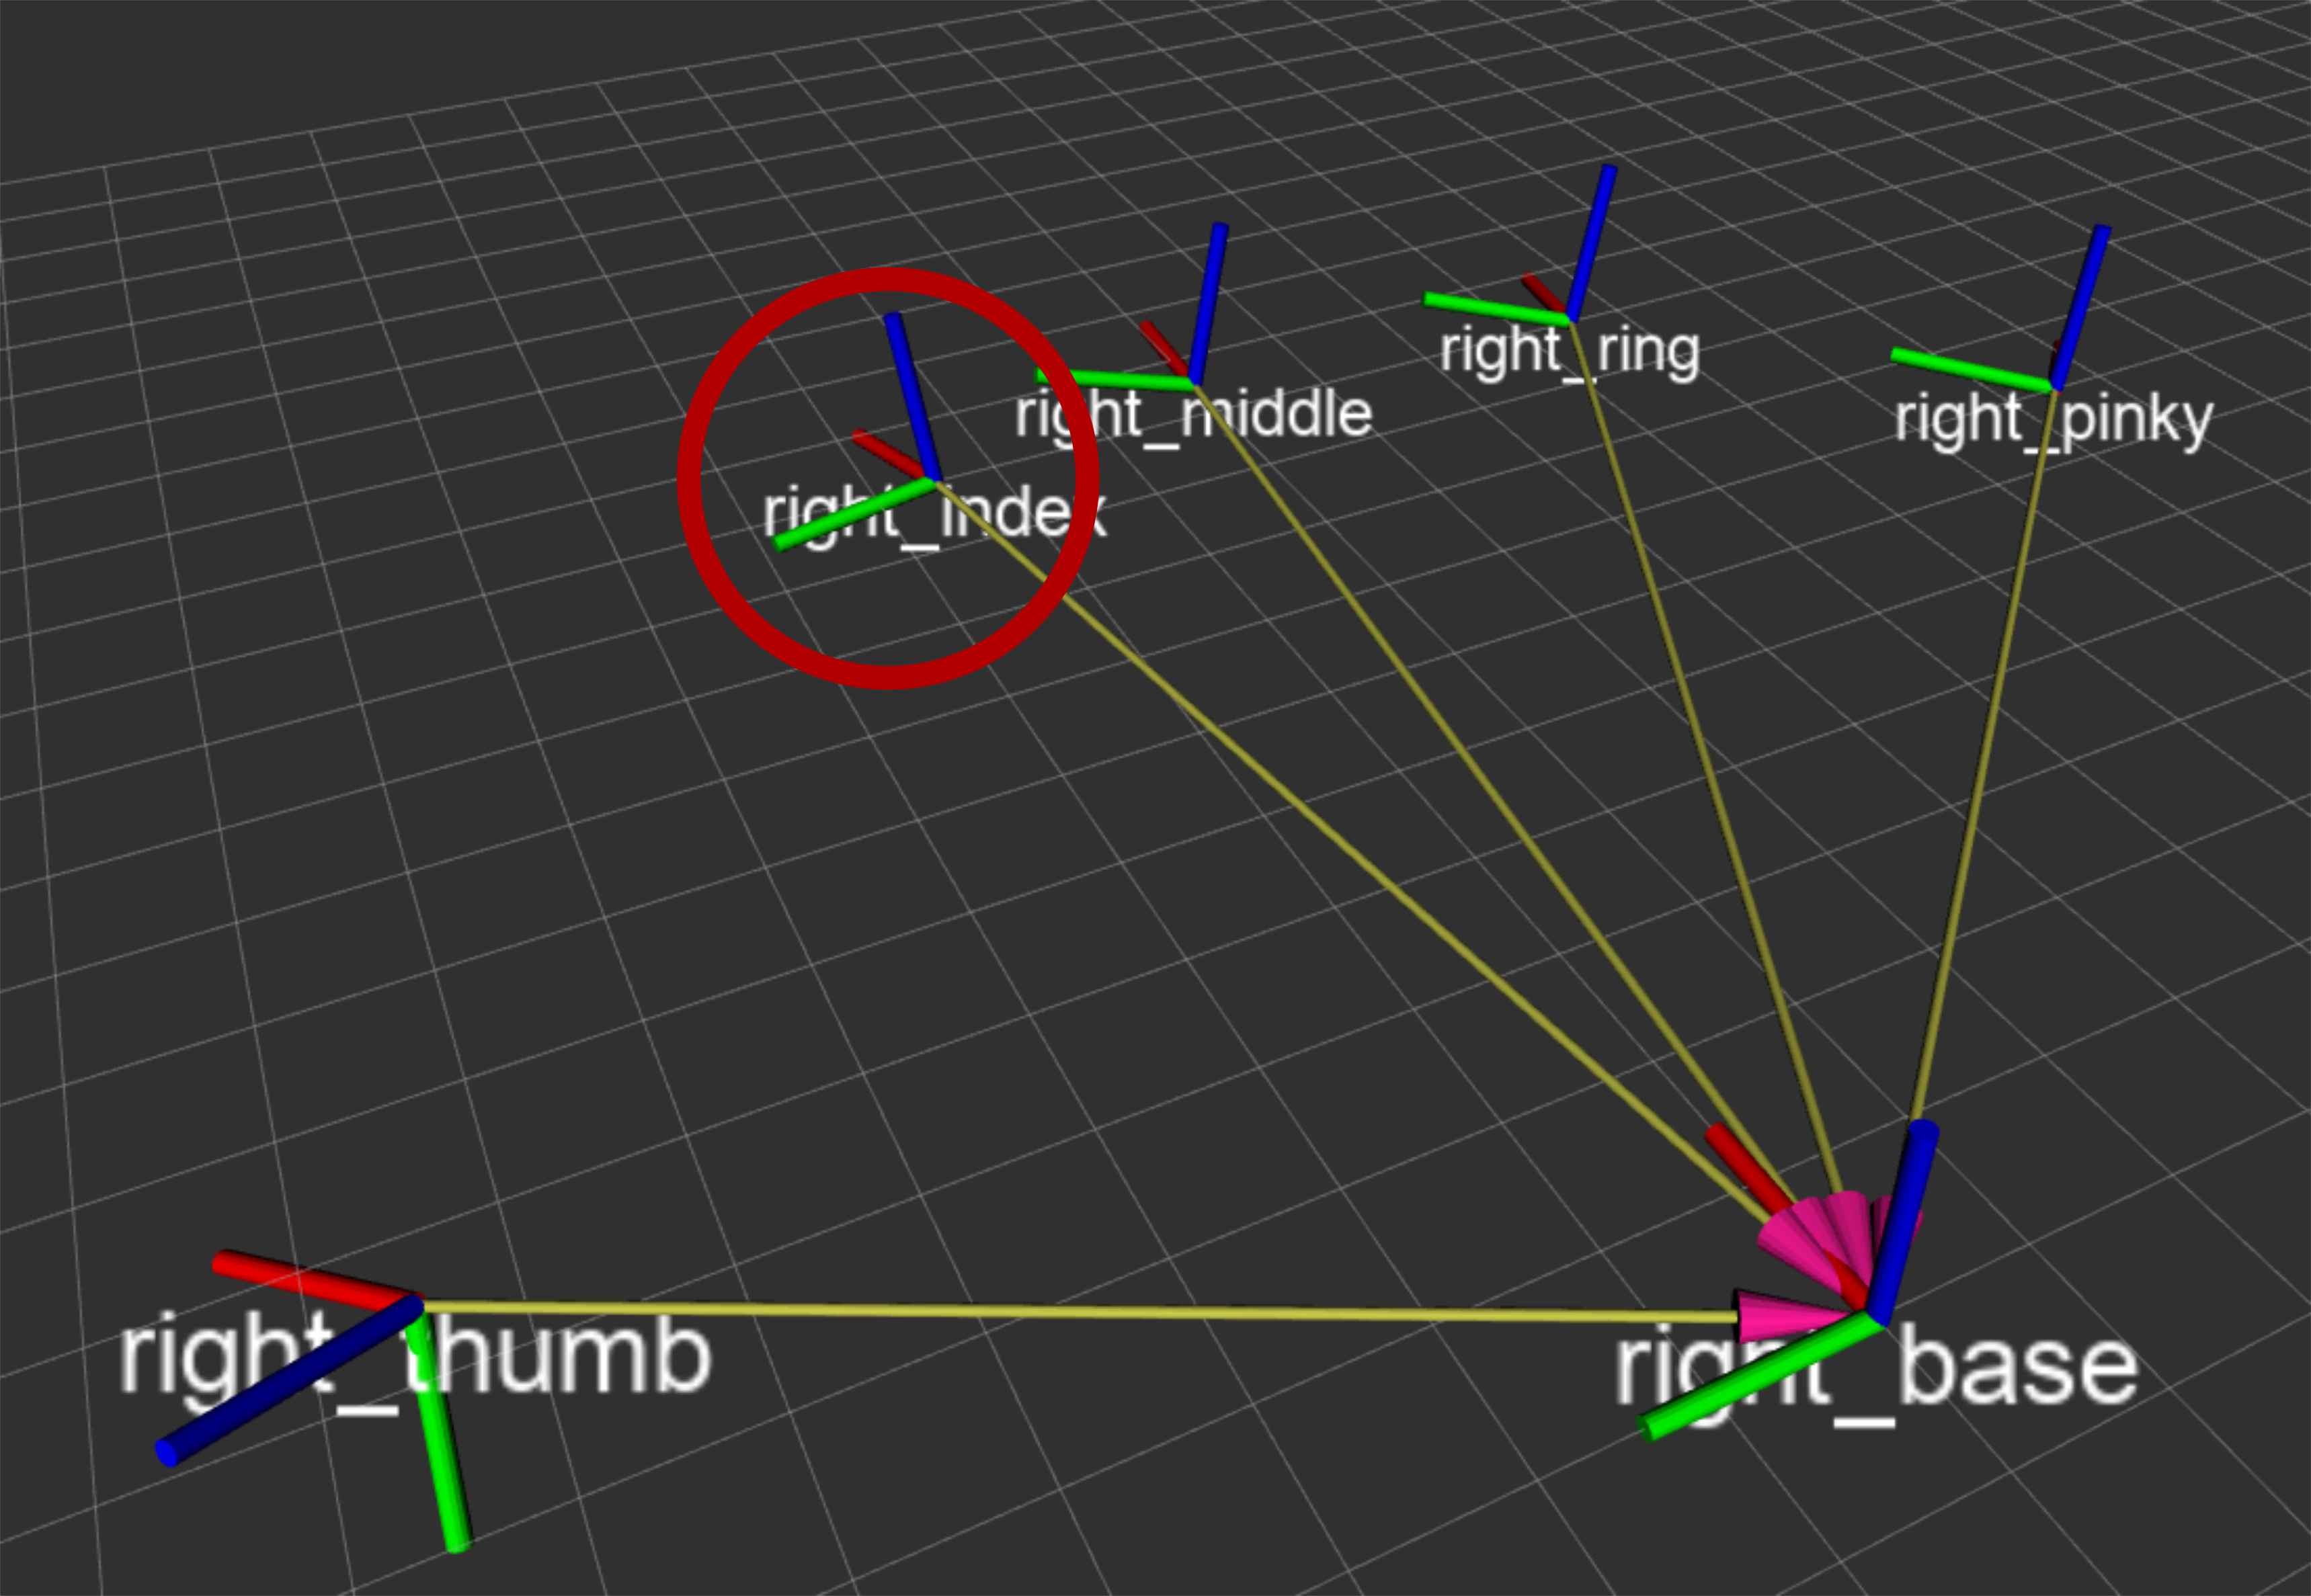
\includegraphics[width=\textwidth]{../common/images/rviz-idle-pose}
                    \caption{Visualization of relative quaternion rotations, idle pose}
                \end{figure}
            }
            \addtocounter{figure}{1}
            \only<3>{
                \begin{figure}
                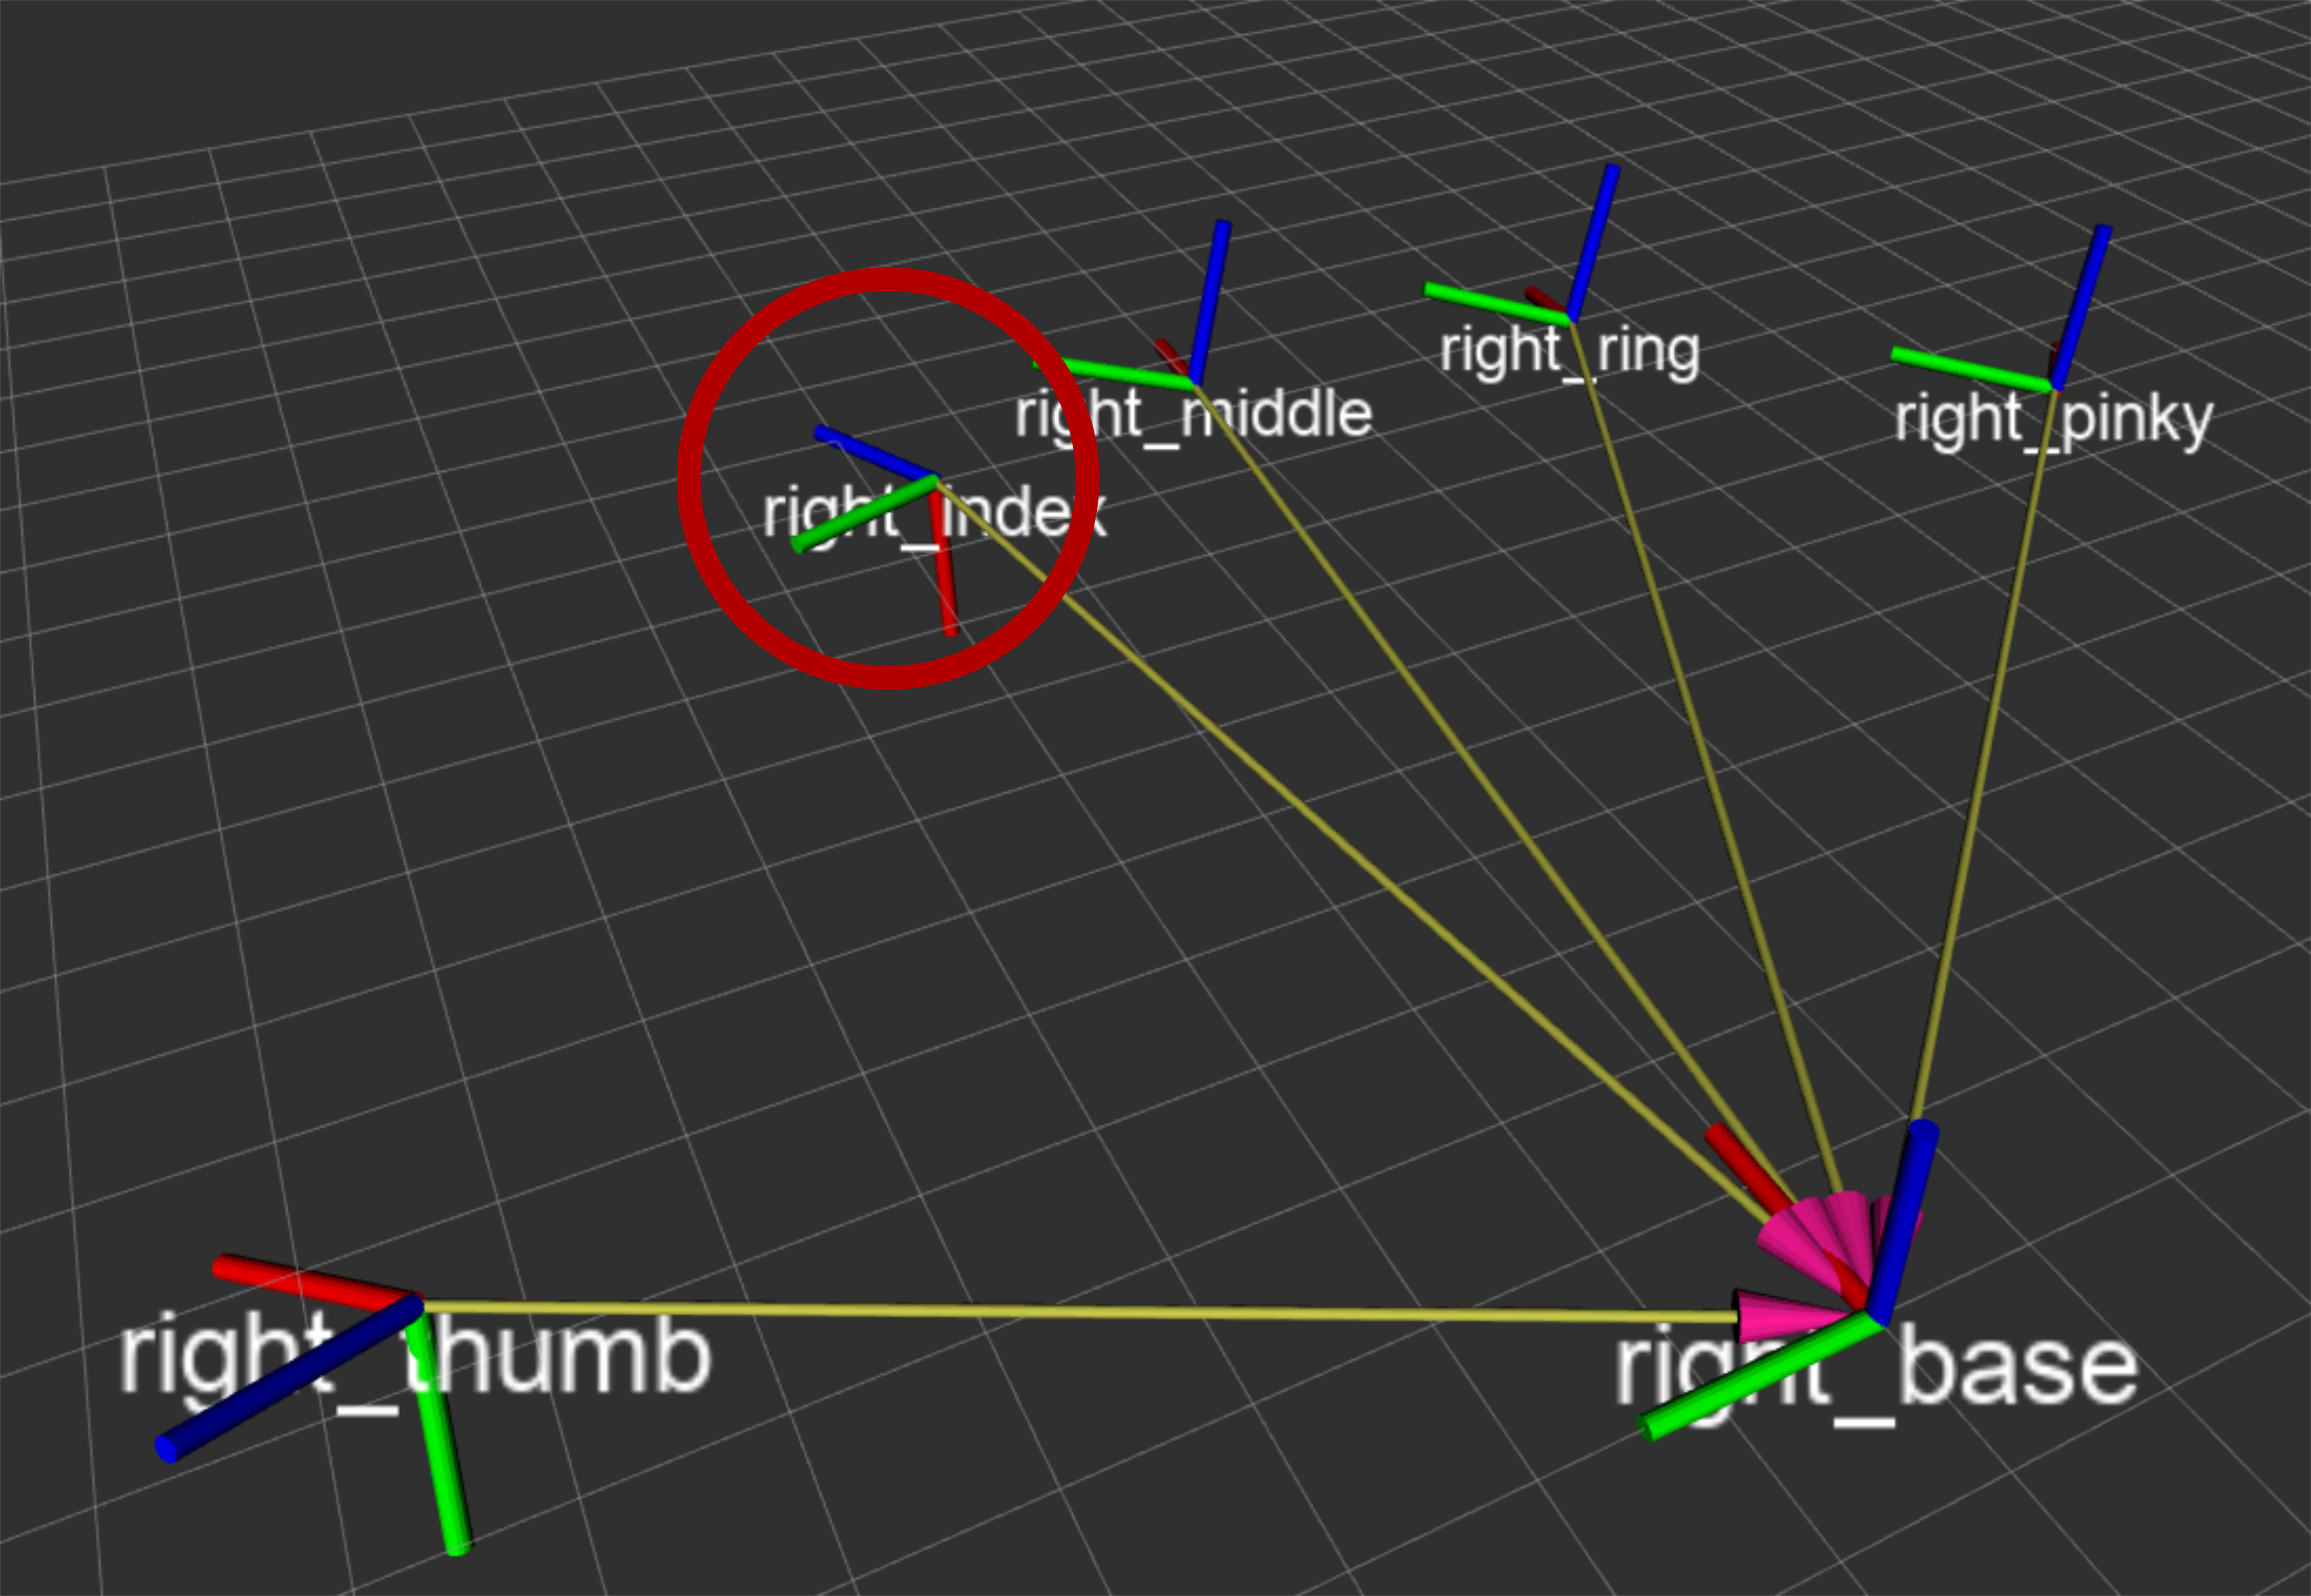
\includegraphics[width=\textwidth]{../common/images/rviz-index-finger-bent}
                    \caption{Visualization of relative quaternion rotations, index finger bent}
                \end{figure}
            }
            \addtocounter{figure}{1}

            \only<4> {
                \begin{figure}
                    \begin{tikzpicture}[
    curve/.style={
        mark=x,
        mark options={thick},
        mark size=3pt,
        thick,
    },
    dot/.style={
        minimum width=4pt,
        minimum height=4pt,
        inner sep=0pt,
        circle,
        draw=secondary,
        thick,
    },
]
    \begin{axis}[
        width=12cm,
        height=6cm,
        axis x line=center,
        axis y line=center,
        xmin=2, xmax=7,
        ymin=2, ymax=5,
        xlabel=Zeit, xtick style={draw=none}, xtick=\empty,
        ylabel=Wert, ytick style={draw=none}, ytick=\empty,
        xlabel near ticks,
        ylabel near ticks,
        legend columns=-1,
        legend style={
            at={(0.5,1.1)},
            anchor=south,
            draw=none,
            font=\scriptsize\bfseries,
            text width=3em,
            text height=1.5ex,
            text depth=.5ex,
        },
    ]
        \addplot[curve,name path=imu-1,color=plot0] plot coordinates {
(-1.90, 1.78) (-1.40, 2.09) (-0.90, 2.32) (-0.40, 2.45) (0.10, 2.58) (0.60, 2.87) (1.10, 3.01) (1.60, 3.01) (2.10, 2.89) (2.60, 2.96) (3.10, 3.05) (3.60, 2.97) (4.10, 2.81) (4.60, 2.77) (5.10, 2.72) (5.60, 2.64) (6.10, 2.49) (6.60, 2.48) (7.10, 2.67) (7.60, 2.81) (8.10, 3.10) (8.60, 3.31) (9.10, 3.48) (9.60, 3.70) (10.10, 3.88) (10.60, 4.05) (11.10, 4.35) (11.60, 4.50)
        };
        \addlegendentry{IMU~1}

        \addplot[curve,name path=imu-2,primary,color=plot1] plot coordinates {
(-1.68, 4.84) (-1.18, 4.89) (-0.68, 4.82) (-0.18, 4.62) (0.32, 4.46) (0.82, 4.13) (1.32, 3.88) (1.82, 3.81) (2.32, 3.71) (2.82, 3.49) (3.32, 3.45) (3.82, 3.24) (4.32, 3.19) (4.82, 3.20) (5.32, 3.24) (5.82, 3.09) (6.32, 2.77) (6.82, 2.62) (7.32, 2.39) (7.82, 2.26) (8.32, 2.32) (8.82, 2.32) (9.32, 2.47) (9.82, 2.55) (10.32, 2.47) (10.82, 2.23) (11.32, 1.92) (11.82, 1.46)
        };
        \addlegendentry{IMU~2}


        \foreach \x/\s [count=\i] in {3.5/2-, 1.5/3-, 5.5/3-, 7.5/3-} {
            \addplot [secondary, name path=line-\i] coordinates{(\x, -0.5) (\x, 5)};

            \path[name intersections={of=imu-1 and line-\i,by=I-\i}];
            \node[dot] at (I-\i) {};

            \path[name intersections={of=imu-2 and line-\i,by=J-\i}];
            \node[dot] at (J-\i) {};
        }

        \draw[secondary,thick,<->]
            (axis cs:3.5,4.6)
                -- node[above] {\tiny{}fester Zeitschritt}
                node[below] {\tiny{}($25$ Hz)}
                (axis cs:5.5,4.6);
    \end{axis}
\end{tikzpicture}

                    \label{fig:interpolation}
                    \caption{Interpolation of the IMU data (simplified)}
                \end{figure}
            }
            \addtocounter{figure}{1}

            \only<5>{
                \vfill\null
                \begin{figure}
                    \centering
                    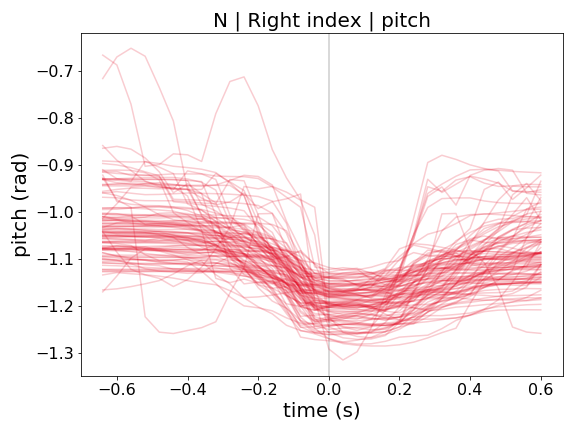
\includegraphics[width=0.8\textwidth]{../common/images/plot-samples-1x1}
                    \caption{Multiple repetitions of the N key stroke, overlayed at the moment of pressing the key (center line); value plotted
                    is extracted relative pitch angle of right index finger.}
                \end{figure}
                \vfill\null
            }
            \addtocounter{figure}{1}

            % Sampling
            % \begin{itemize}
            %     \item 25 Hz timesteps
            %     \item 16 timesteps per sample
            %     \item key stroke in center
            %     \item 100 samples per epoch
            % \end{itemize}
        \end{column}
    \end{columns}

    \note{
        \begin{enumerate}
            \item Quat:
            \begin{itemize}
                \item absolute orientation (heading north)
                \item goal: independent of direction
                \item solution: use relative quaternions (handbase)
                \item hand relative to moving average
                \item $$q_{rel} = q_{abs} \cdot inv(q_{abs,parent})$$
            \end{itemize}
            \item interpolate
            \begin{itemize}
                \item fixed timesteps
                \item need all imu data
            \end{itemize}
            \item sampling
            \begin{itemize}
                \item time 0 : keystroke
                \item 8 timesteps before + after
                \item visualization: many keystrokes, angles \textbf{yaw, pitch}
            \item acceleration (linear acceleration)
            \item gyroscope (angular velocity (rotate speed))
            \item (spherical) linear interpolation $\rightarrow$ see next slide
            \end{itemize}
        \end{enumerate}
    }
\end{frame}

\begin{frame}{Preprocessing and Sampling}{Real Preprocessed Data}
    \phasekeyboard{1}
    \vspace{-1em}
    \begin{figure}
        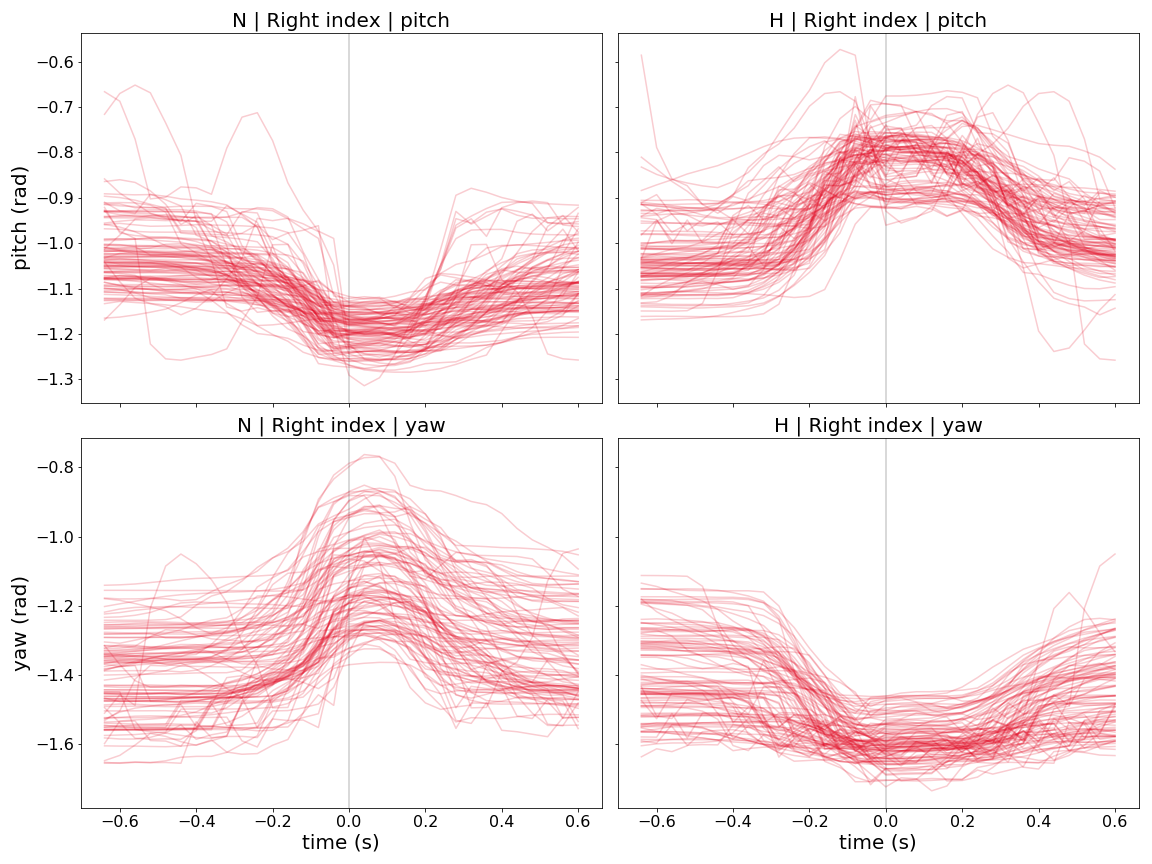
\includegraphics[width=0.65\textwidth]{../common/images/plot-samples-2x2}
        \label{fig:our_data}
        \caption{Multiple repetitions of N (\emph{left}) and H (\emph{right})
        key strokes, overlayed at the moment of pressing the key (center line);
        value plotted is extracted relative pitch (\emph{top})/yaw
        (\emph{bottom}) angles of right index finger.}
    \end{figure}

    \notes{
        \item we tried to visualize what we got
        \item 1 finger, left: N, right: H
        \item Quaternion: yaw, pitch
        \begin{itemize}
            \item quat is enough, acc and gyro data can be used additionally $\rightarrow$ requires more training
            \item finger cant roll relative to hand $\rightarrow$ no roll necessary (only hand)
        \end{itemize}
        \item actual moment of keystroke!
        \item hill, valley!
        \item visibly different --> detectible!!
    }
\end{frame}

\subsection{Convolutional Neural Networks}
\begin{frame}[fragile]{Convolutional Neural Networks}{Convolution and Pooling}
    \begin{figure}
        \begin{tikzpicture}
    \matrix(start)[
        matrix of nodes,
        inner sep=0pt,
        draw,
        nodes={
            inner sep=0pt,
            text width=.5cm,
            align=center,
            minimum height=.5cm,
            draw,
        }
    ]{
       5  & 2 & 3 & 8 \\    0 & |[fill=primary!25]|{1} & 2 & 6 \\    4 & 8 & 5 & 4 \\    1 & 7 & 1 & 7\\};

    \matrix(filter0)[
        inner sep=0pt,
        draw,
        label=above:{\tiny{}Filter 0},
        opacity=0.5,
        above right=-0.2cm and 0.8cm of start,
        matrix of nodes,
        nodes={
            inner sep=0pt,
            text width=.5cm,
            align=center,
            minimum height=.5cm,
            draw,
        },
    ]{
        0 & 1 & 0 \\    0 & 1 & 0 \\    0 & 1 & 0 \\};
    \matrix(filterN)[
        inner sep=0pt,
        draw,
        label=above:{\tiny{}Filter N},
        opacity=0.5,
        below right=-0.2cm and 0.8cm of start,
        matrix of nodes,
        nodes={
            inner sep=0pt,
            text width=.5cm,
            align=center,
            minimum height=.5cm,
            draw,
        },
    ]{
        0 & 0 & 1 \\    0 & 1 & 0 \\    1 & 0 & 0 \\};

    \node (rect) at (-0.25, 0.25) [draw=primary,line width=0.6mm,minimum width=1.5cm,minimum height=1.5cm] {};
    \draw[->, thick, primary] (rect) -- (filter0);
    \draw[->, thick, primary] (rect) -- (filterN);

    \matrix(conv0)[
        matrix of nodes,
        inner sep=0pt,
        draw,
        right=of filter0,
        label=above:{\tiny{Feature Map 0}},
        nodes={
            inner sep=0pt,
            text width=.5cm,
            align=center,
            minimum height=.5cm,
            draw,
        }
    ]{
        5 & 3 & 5 & 14 \\    9 & |[fill=primary!25]|{11} & 10 & 18 \\    5 & 16 & 8 & 17 \\    5 & 15 & 6 & 11\\};

    \matrix(convN)[
        matrix of nodes,
        inner sep=0pt,
        draw,
        right=of filterN,
        label=above:{\tiny{}Feature Map N},
        nodes={
            inner sep=0pt,
            text width=.5cm,
            align=center,
            minimum height=.5cm,
            draw,
        }
    ]{
        5 & 2 & 4 & 10 \\    2 & |[fill=primary!25]|{8} & 18 & 11 \\    5 & 11 & 18 & 5 \\    9 & 12 & 5 & 7\\};

    \node (rect2) at ($(conv0) + (-0.5, 0.5)$) [draw=orange,line width=0.6mm,minimum width=1cm,minimum height=1cm] {};
    \node (rect2) at ($(convN) + (-0.5, 0.5)$) [draw=orange,line width=0.6mm,minimum width=1cm,minimum height=1cm] {};
    \matrix(pool0)[
        inner sep=0pt,
        draw,
        label=above:{\tiny{}Pool 0},
        right=of conv0,
        matrix of nodes,
        nodes={
            inner sep=0pt,
            text width=.5cm,
            align=center,
            minimum height=.5cm,
            draw,
        },
    ]{
        |[fill=orange!25]|{11} & 18 \\    16 & 17 \\};
    \matrix(poolN)[
        inner sep=0pt,
        draw,
        label=above:{\tiny{}Pool N},
        right=of convN,
        matrix of nodes,
        nodes={
            inner sep=0pt,
            text width=.5cm,
            align=center,
            minimum height=.5cm,
            draw,
        },
    ]{
        |[fill=orange!25]|{8} &  18\\    12 & 18 \\};
    % \draw(rect)[primary, line width=0.65mm] (-1,-0.5) rectangle (0.5,1);
    \draw[->, line width=1pt, primary,bend angle=20] (filter0.east |- conv0-2-2.north west) to[bend left] (conv0-2-2.north west);
    \draw[->, line width=1pt, primary,bend angle=20] (filterN.east |- convN-2-2.north west) to[bend left] (convN-2-2.north west);
    \draw[->, line width=1pt, orange,bend angle=20] (conv0-2-2.east |- pool0-1-2.north west) to[bend left] (pool0-1-1.north west);
    \draw[->, line width=1pt, orange,bend angle=20] (convN-2-2.east |- poolN-1-2.north west) to[bend left] (poolN-1-1.north west);
    \node[font=\Large] at ($(filter0)!0.45!(filterN)$) {$\vdots$};
    % \path   (rect) edge              node {} (filter0)
            % (rect) edge              node {} (filterN);

    \node[font=\Large] at ($(conv0)!0.45!(convN)$) {$\vdots$};
\end{tikzpicture}

        \label{fig:cnn}
        \caption{Feature Extraction with CNN}
    \end{figure}

    \notes{
        \item convolute (element wise multiplication)
        \item pool (max)
        \item filters (50)
        \item 3 x 3 x 50
        \item convolute, pool..
        \item fully connected layer as classifier
    }
\end{frame}

\begin{frame}[fragile]{Convolutional Neural Networks}{Our Implementation}
    \vspace{-1em}
    \begin{tikzpicture}[
    node distance=5mm,
    io/.style={
        flowchart node,
        minimum height=0.5cm,
        text width=1cm,
        minimum width=0cm,
    },
    arrow/.style={
        flowchart arrow,
    },
    arrow/.style={
        ->,
        >=stealth',
        shorten >=1pt,
        auto,
        semithick,
    },
    layer/.style={
        draw,
        minimum width=0.9cm,
        minimum height=6cm,
    },
    bend angle=15,
    every state/.style={
        fill=white,
        minimum size=3mm,
        inner sep=0pt,
        node distance=7mm,
    },
    steplabel/.style={
        font=\scriptsize,
        above,
        rotate=90,
        anchor=west,
    },
]
    \node[io] (data) {1 @\\16 x 24};
    \node[io, right=of data] (conv1)  {50  @\\$16 \times 24$};
    \node[io, right=of conv1] (pool1) {50   @\\$8 \times 12$};
    \node[io, right=of pool1] (conv2) {50 @\\$8 \times 12$};
    \node[io, right=of conv2] (pool2) {50 @\\$4 \times 6$};
    \node[io, right=of pool2] (hidden) {Hidden\\Layer};
    \node[io, right=of hidden] (out) {Output\\Layer};

    \draw [arrow] (data)   -- node[steplabel] {conv 1} (conv1);
    \draw [arrow] (conv1)  -- node[steplabel] {pool 1} (pool1);
    \draw [arrow] (pool1)  -- node[steplabel] {conv 2} (conv2);
    \draw [arrow] (conv2)  -- node[steplabel] {pool 2} (pool2);
    \draw [arrow] (pool2)  -- node[steplabel] {dense} (hidden);
    \draw [arrow] (hidden) -- node[steplabel] {dense} (out);
\end{tikzpicture}

    \notes{
        \item each key has same amount of samples
        \item one sample = one keystroke
        \item filter randomly initialized
        \item filter are learned!
        \item matrix with numbers instead of color scheme
        \item 2 x convolute and pooling
        \item MSE: $(1/n)*\sum_{n=0}^{N} (pred - act)^2$
            % \begin{itemize}
            %     \item Input: relative angles of quaternions
            %      \item Hand Imu: relative to last position
            %     \item 50 3x3 Filter
            %     \item 2 Iterations
            %     \item fully connected layer
            %     \item N units in output layer ($N=count of keys$)
            %     \item costfunction: Mean Squared Error
            % \end{itemize}
    }
\end{frame}
\subsection{Evaluating Predictions}


\addtocontents{toc}{\newpage}


\section{Experiments}

\subsection{Phase 0~\textendash{}~Pipeline Setup}
\begin{frame}[fragile]{Phase 0~\textendash{}~Pipeline Setup}
    \begin{columns}[T]
        \begin{column}{0.56\textwidth}
            \begin{figure}
                \begin{minted}[style=friendly,fontsize=\scriptsize]{c}
imu_ids: [0, 1, 2, 3, 4, 5]
key_codes: [21, 22, 23, 34, ...]
sequence_length: 16

epochs: 0 //infinite
learning_rate: 0.002
batch_size: 100
sampling_rate: 25

network_type: cnn2d
cost_function: mse

convolution_n_filters: 50
convolution_filter_size: [3, 3]
convolution_n_pairs: 2
convolution_arr_dense: [10]
                \end{minted}
% training_ratio: 0.8
% output_threshold: 0.5
% n_hidden: 20
               \label{fig:config}
               \caption{Example of a configuration file (truncated)}
            \end{figure}
        \end{column}
        \begin{column}{0.38\textwidth}
            \begin{itemize}
                \item easily adjustable
                \item repeatable experiments
            \end{itemize}
        \end{column}
    \end{columns}
    \notes{
        \item Theano is a scientific mathematical library
        \begin{itemize}
            \item large scale calculations
            \item often numpy arrays
        \end{itemize}
        \item Lasagne is a ML-Framework based on Theano
        \begin{itemize}
            \item focused on Neural Networks
        \end{itemize}
    }
\end{frame}


\subsection{Phase 1~\textendash{}~Slow Single Finger}
\begin{frame}[fragile]{Phase 1~\textendash{}~Slow Single Finger}{Overview}
    \phasekeyboard{1}
    1 finger, 2 keys

    \pause
    \vspace{2em}
    Goals:
    \begin{itemize}
        \item detect keystrokes, ignore idle pose
        \item distinguish between close keys
        \item evaluate the configuration of the CNN
    \end{itemize}

    \notes{
        \item index finger moving between N, H
        \item pauses
        \item mostly detect pressed N
        \item always ignore H
    }
\end{frame}

\begin{frame}[fragile]{Phase 1~\textendash{}~Slow Single Finger}{Accuracy and Cost Function}
    \phasekeyboard{1}
        \begin{figure}
            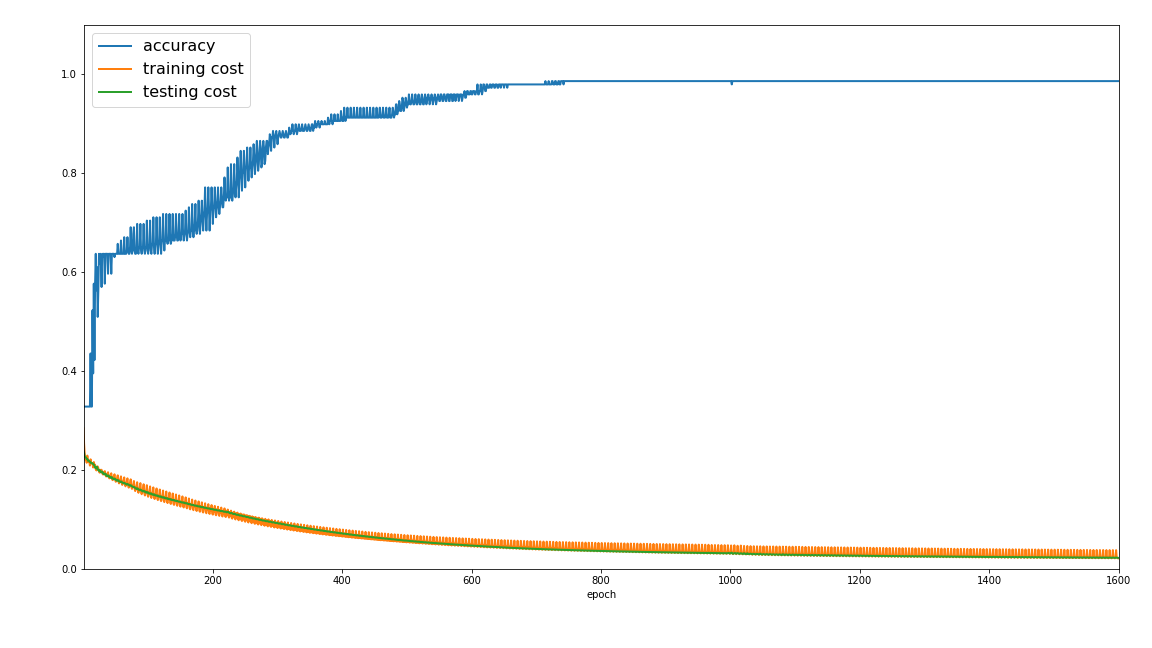
\includegraphics[width=0.85\textwidth]{../common/images/phase-1}
            \label{fig:phase11}
            \caption{Test results in the first $1 600$ epochs of learning phase 2}
        \end{figure}
    \notes{
        \item $1600$ epochs
        \item accuracy: amount of correctly classified samples
        \item 1 epoch: 1 batch
        \item 1 batch: 100 samples
        \item 1 sample: 1keystroke or nokey: 16 timesteps
    }
\end{frame}

\subsection{Phase 2~\textendash{}~Slow Multiple Fingers}
\begin{frame}[fragile]{Phase 2~\textendash{}~Slow Multiple Finger}{Overview}
    \phasekeyboard{2}
    3 fingers, 10 keys

    \pause
    \vspace{2em}
    Goals:
    \begin{itemize}
        \item distinguish between fingers
        \item handle hand movement
    \end{itemize}
\end{frame}

\begin{frame}[fragile]{Phase 2~\textendash{}~Slow Multiple Fingers}{Accuracy and Cost Function}
    \phasekeyboard{2}
    \begin{figure}
        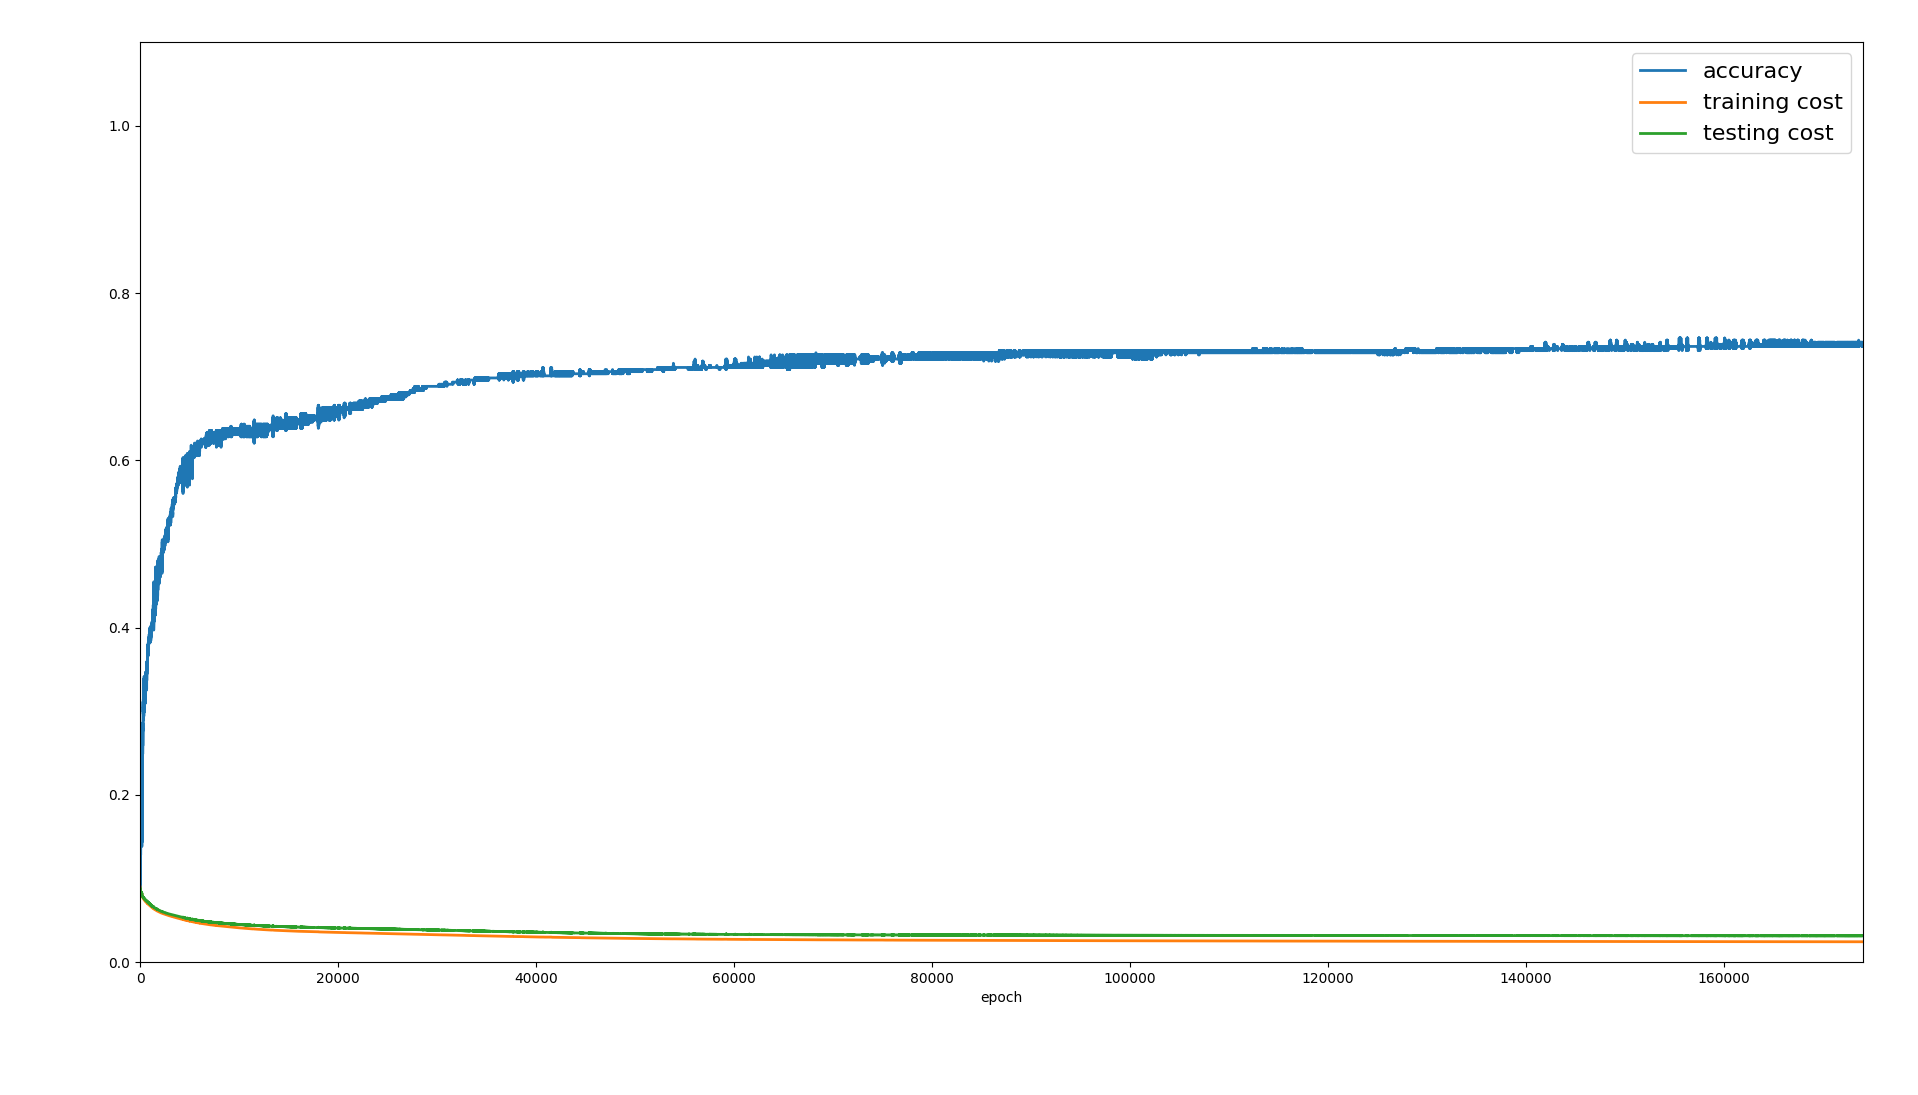
\includegraphics[width=0.85\textwidth]{../common/images/phase-2}
        \label{fig:phase21}
        \caption{Test results in the first $160 000$ epochs of learning phase 2}
    \end{figure}
    \notes{
        \item over $160000$ epochs $\rightarrow$ much more epochs necesarry
        \item accuracy only near 70\%
    }
\end{frame}

\subsubsection{Evaluation of Predictions}
\begin{frame}{Phase 2~\textendash{}~Slow Multiple Fingers}{Evaluation of Predictions}
    \phasekeyboard{2}
    \begin{figure}
        \scalebox{0.9}{
            \pgfkeys{/pgf/declare function={rescale(\x) = (\x*2-1)^3*0.5+0.5;}}

\begin{tikzpicture}[
    square/.style={
        inner sep=0pt,
        rectangle,
        minimum width=1cm,
        minimum height=0.5cm,
        anchor=north west,
    },
    every node/.style={
        font=\scriptsize,
    },
]
    % \node[inner sep=2pt,circle,fill=green] at (0, 0) {};
    \node[inner sep=0pt,rectangle,anchor=south east,rotate=90,minimum width=5cm,minimum height=0.5cm,draw,xshift=0.5\pgflinewidth,thick]
        at (0, -0.5) {\bfseries{}Actual};
    \node[inner sep=0pt,rectangle,anchor=south west,minimum width=10cm,minimum height=0.5cm,draw,xshift=-0.5\pgflinewidth,thick]
        at (1, 0) {\bfseries{}Predicted};

    \foreach \row [count=\y] in {{0,13,5,9,5,121,2,6,3,0},{0,175,0,0,0,0,0,0,0,0},{0,1,167,0,0,0,0,0,0,0},{0,0,0,181,0,0,0,0,0,0},{0,1,5,0,1,169,0,0,0,0},{0,0,1,0,1,215,0,3,0,0},{0,0,0,0,0,0,167,0,0,0},{0,0,0,0,0,0,0,180,0,0},{0,0,0,0,0,0,0,0,190,0},{0,0,0,0,4,178,1,0,0,0}} {
        \foreach \v [count=\x] in \row {
            \pgfmathsetmacro{\tmp}{\v/215.0}
            \pgfmathtruncatemacro{\back}{rescale(\tmp)*100}
            \pgfmathtruncatemacro{\fore}{(\tmp>0.5)*100}
            \node[square,fill=black!\back!white,text=white!\fore!black] at (\x,-\y*0.5) {$\v$};
        }
    }

    \foreach \key [count=\i] in {$\emptyset$,Y,U,G,H,J,B,N,M,\textvisiblespace} {
        \node[square] at (0, -(\i*0.5) {\bfseries\key};
        \node[square] at (\i, 0) {\bfseries\key};
    }

    \foreach \i in {2,...,10} {
        \draw[draw,dotted] (\i, 0) -- (\i, -5.5);
        \draw[draw,dotted] (0, -\i*0.5) -- (11, -\i*0.5);
    }

    \foreach \i in {1,11} {
        \draw[draw,thick] (\i, 0) -- (\i, -5.5);
        \draw[draw,thick] (0, -\i*0.5) -- (11, -\i*0.5);
    }
\end{tikzpicture}

        }
        \label{fig:confusion-matrix}
        \caption{Confusion matrix\citep{poole-artificial-intelligence}. From this we calculate the accuracy and per key recall \& precision \citep{davis2006}}
    \end{figure}

    \note{
        \begin{itemize}
            \item left : actual, right: predicted
            \item wrong classificated:
            \begin{itemize}
                \item no key as j
                \item h as j
                \item space as j
            \end{itemize}
            \item apple keyboard doesnt need much finger movement to press key
            \item $\rightarrow$ mechanical keyboard??!
            \item additional stuff:
            \begin{itemize}
                \item recall precision needs to be balenced (--> imbalanced data!!)
                \item recall: RECALL :D avoid FN!
                \item precision: avoid FP
                \item accuracy: TP / ALL
                \item recall:  TP/ TP +  FN how many relevant items (TP + FN) are selected
                \item precision: TP/ TP + FP how many selected items are relevant
            \end{itemize}
        \end{itemize}
    }
\end{frame}

\subsection{Phase 3~\textendash{}~Fast Typing}
\begin{frame}[fragile]{Phase 3~\textendash{}~Fast Typing}{Overview}
    \phasekeyboard{3}
    5 fingers, 27 keys

    \pause
    \vspace{2em}
    Goals:
    \begin{itemize}
        \item recognizing every righthand key stroke
        \item achieve high accuracy
        \item learn a robust model
        \item fluent typing
    \end{itemize}

    \notes{
        \item future (we did not do this yet)
        \item next step: online learning
        \item modification of movements
    }
\end{frame}

\section{Demo}

\begin{frame}{Demo}{The Glove}
    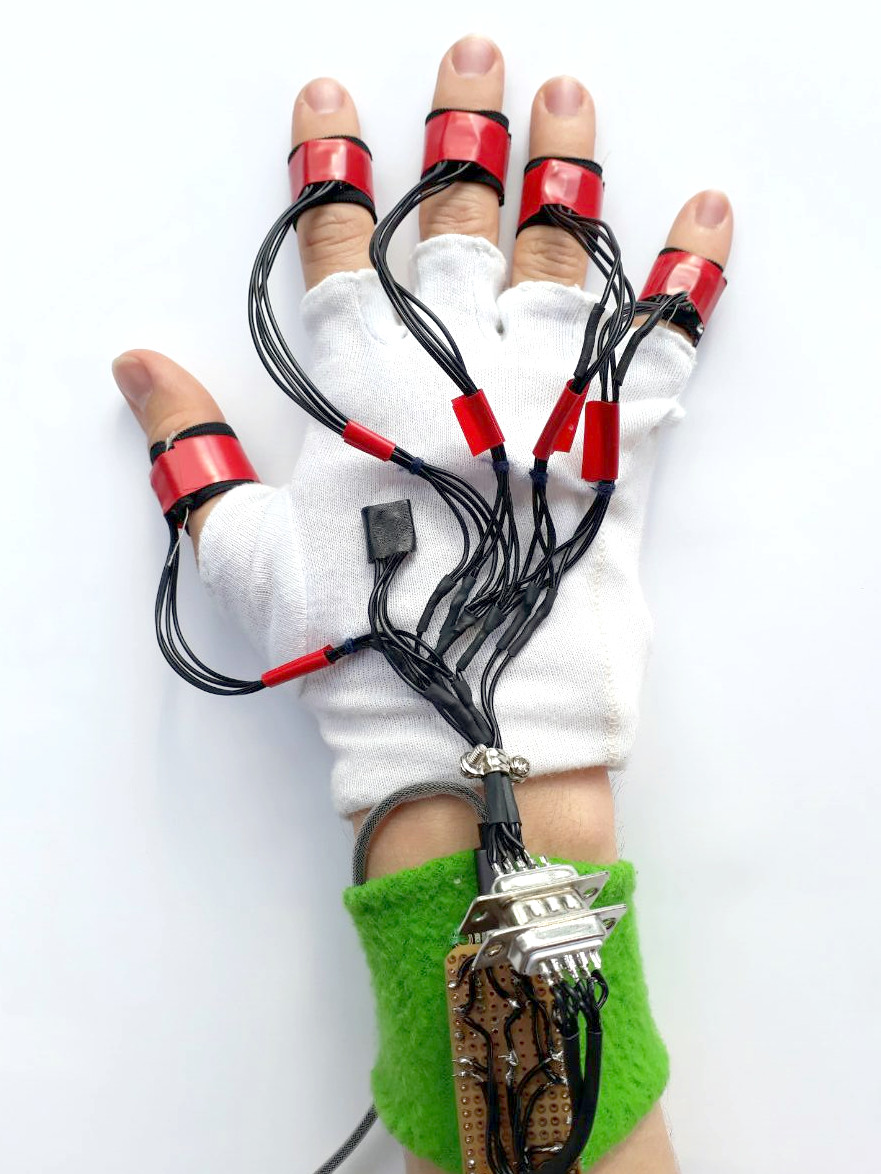
\includegraphics[height=0.75\textheight]{../common/images/glove-top}
    \hfill
    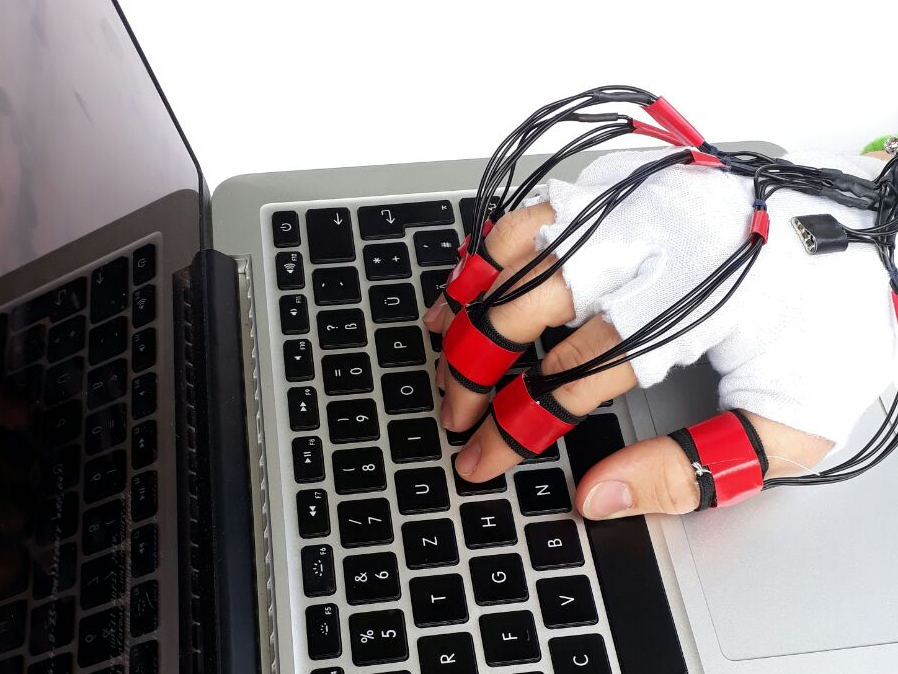
\includegraphics[height=0.4\textwidth]{../common/images/glove-live}
\end{frame}

\begin{frame}{Demo}{Backup Videos}
    \vfill%
    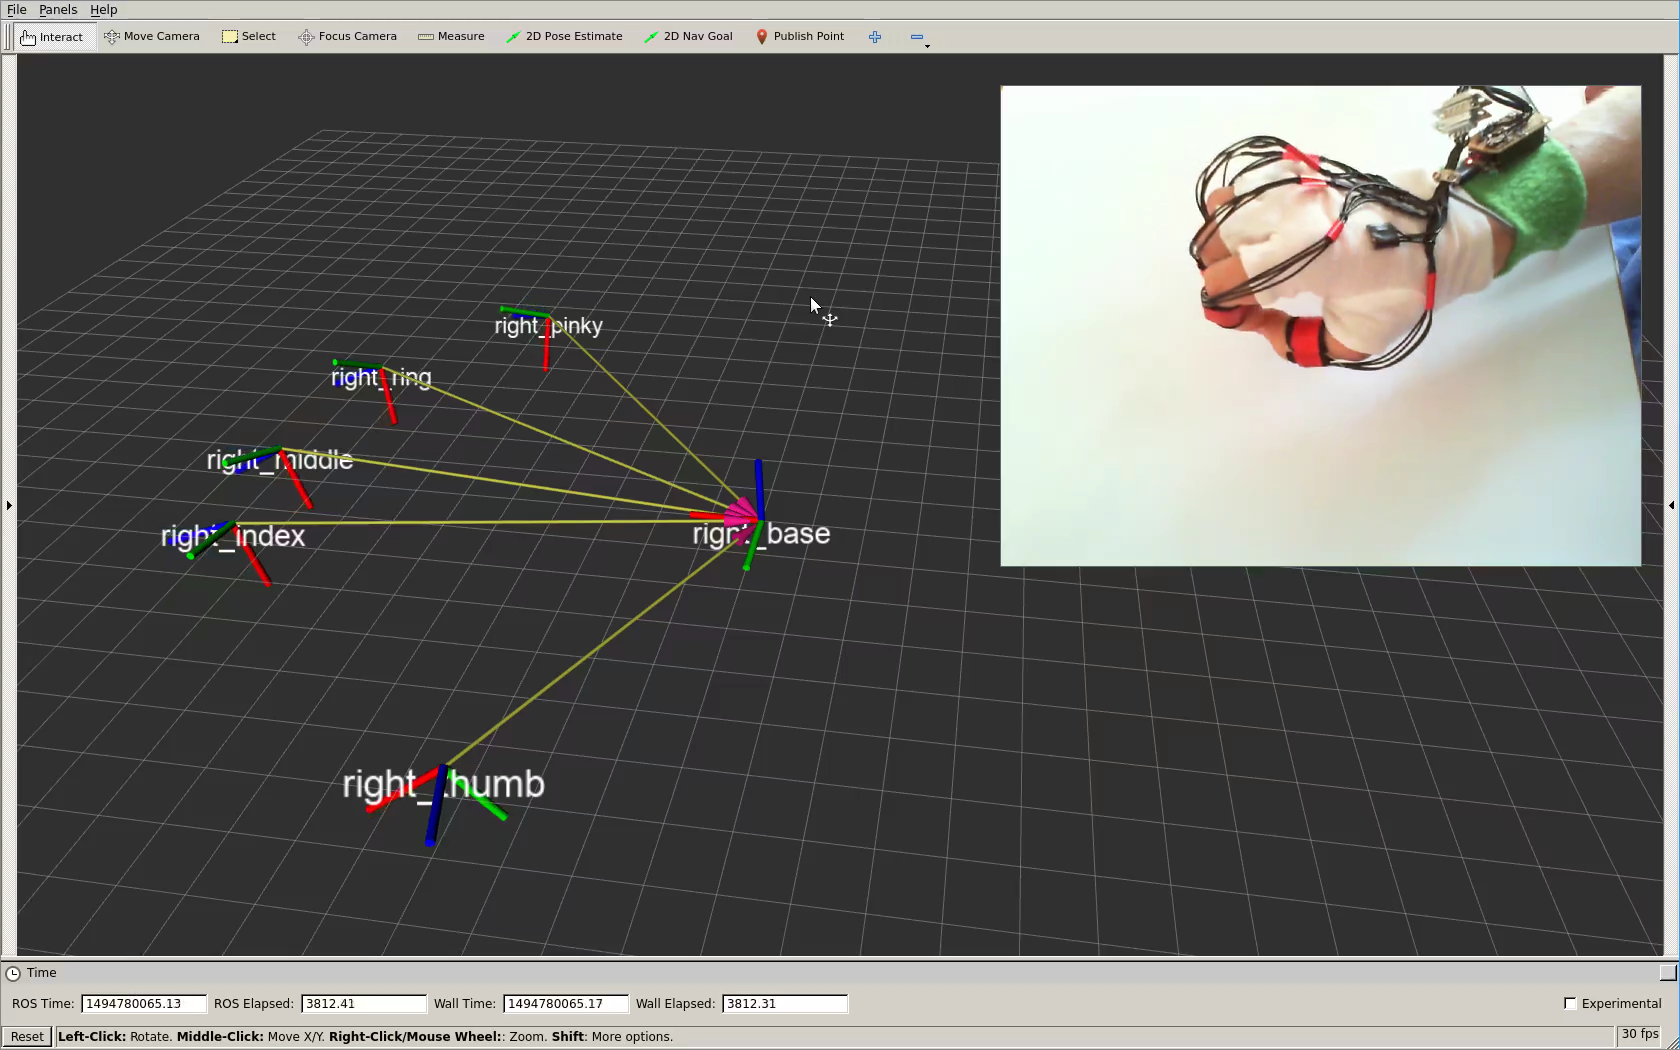
\includegraphics[width=0.49\textwidth]{../demo/01-rviz}
    \hfill
    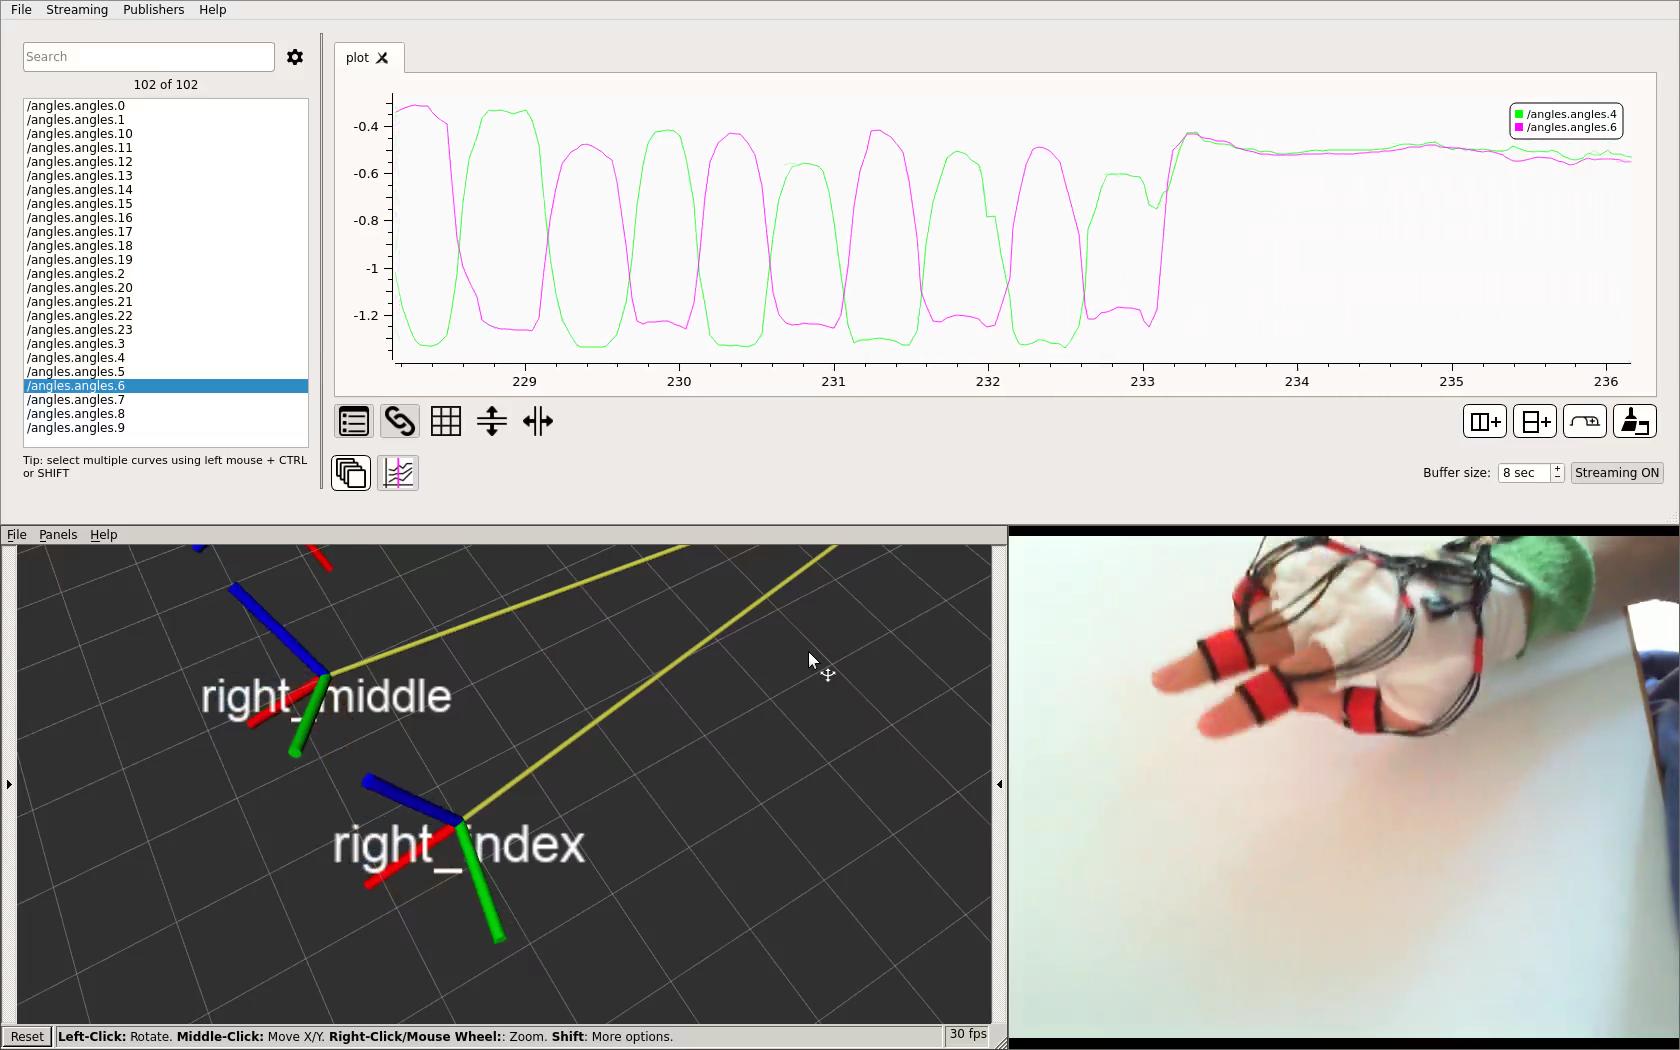
\includegraphics[width=0.49\textwidth]{../demo/02-plotjuggler}
\end{frame}

\section{Conclusion}
\subsection{Results}
% \begin{frame}{Results System Design}
%     \centering
%     \vfill
%     \begin{tabular}{r | l}
%         Successes & Improvements to make \\
%         \hline
%         the glove is non-obstructive & robustness \\
%         performance good enough for prototype & generalization to different hand types \\
%         architecture proved suitable & one piece glove \\
%     \end{tabular}
% \end{frame}

\begin{frame}{Results System Design}
    \begin{block}{Goal (Reminder)}
        Design a system for recording characteristic hand movements of typing
        and the corresponding input.
    \end{block}
    \pause
    \vfill\null
    \begin{columns}[T]
        \begin{column}{0.5\textwidth}
            \textbf{Successes}
            \begin{itemize}
                \item the architecture proved suitable
                \item the glove is non-obstructive
                \item performance is good enough for a prototype
            \end{itemize}
        \end{column}
        \begin{column}{0.5\textwidth}
            \textbf{Improvements}
            \begin{itemize}
                \item gyro clipping
                \item single robust glove
                \item generalization to different hand types
            \end{itemize}
        \end{column}
    \end{columns}
\end{frame}

\begin{frame}{Results Machine Learning}
    \begin{block}{Goal (Reminder)}
        Define an approach for utilizing machine learning to map the recorded
        data back to the keyboard input.
    \end{block}
    \pause
    \vfill\null
    \begin{columns}[T]
        \begin{column}{0.5\textwidth}
            \textbf{Successes}
            \begin{itemize}
                \item slow typing can be distinguished
                \item preprocessing helps the learning progress
                \item CNNs can distinguish between different keys
            \end{itemize}
        \end{column}
        \begin{column}{0.5\textwidth}
            \textbf{Improvements}
            \begin{itemize}
                \item better accuracy
                \item reduce delay
                \item detect holding a key
                \item detect different modes $\rightarrow$(non-)writing position
            \end{itemize}
        \end{column}
    \end{columns}

    \notes{
        \item fscore, recall, precision
        \item delay
            \begin{itemize}
                \item keystroke in middle
                \item 8 timesteps before and after
            \end{itemize}
        \item learn on more data (accel, gyro..)
            \begin{itemize}
                \item learn more about hand position not only orientation
            \end{itemize}
    }
\end{frame}
% \begin{frame}{Results}{Successes System Design}
%     \begin{itemize}
%     \end{itemize}
% \end{frame}
% \begin{frame}{Results}{Successes Machine Learning}
%         \begin{itemize}
%         \end{itemize}
% \end{frame}
% \begin{frame}{Results}{Failures}
%     \begin{itemize}
%         \item RNN did not work
%         \begin{itemize}
%             \item therefore we did preprocessing and looked at the structure of our data
%         \end{itemize}
%         \item huge delays
%         \begin{itemize}
%             \item can be reduced by using another time step window around keypress event
%         \end{itemize}
%         \item cannot detect holding key
%         \begin{itemize}
%             \item use all imu data to get a better understanding of actual hand position
%             \item learn key releases
%         \end{itemize}
%     \end{itemize}
% \end{frame}

\subsection{Outlook}
\begin{frame}{Outlook}
    \begin{block}{Goal (Reminder)}
        Evaluate the quality of such mapping and discuss whether this principle
        could be turned into a working keyboard alternative.
    \end{block}
    \pause
    \vfill\null
    \begin{itemize}
        \item reduce delay, remove lookaheads
        \item increase prediction quality
        \item two hands
        \item generalize glove \& model
        \item implement online learning
        \item better hand pose reconstruction for more use cases
        % \item publish schematics and instructions for building the glove
    \end{itemize}
\end{frame}

\appendix
\begin{frame}[allowframebreaks]{References}
    \renewcommand*{\bibfont}{\scriptsize}
    \printbibliography
\end{frame}

\begin{frame}[plain]
   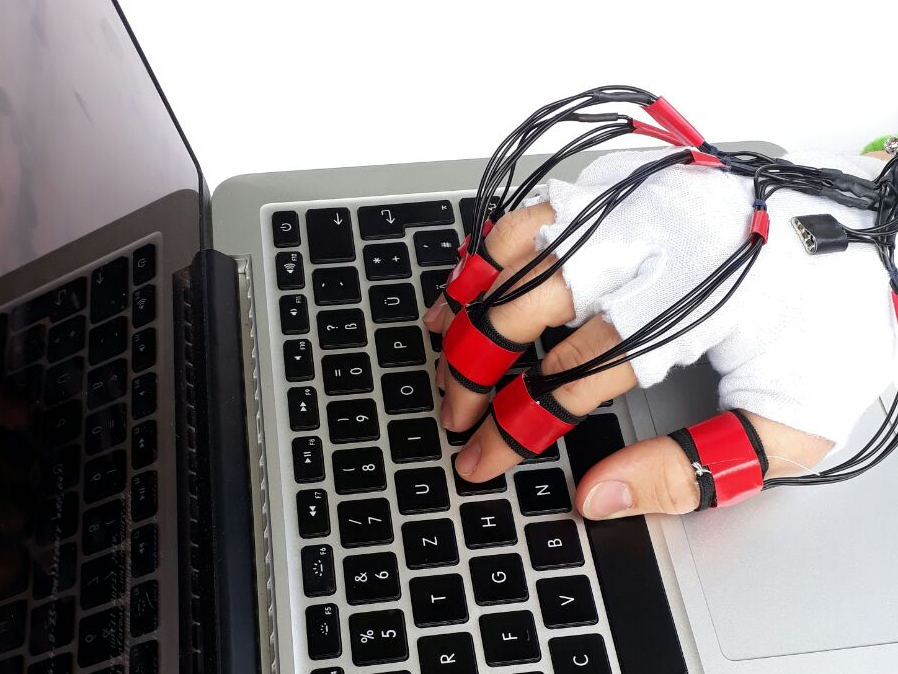
\includegraphics[width=0.9\textwidth]{../common/images/glove-live}
\end{frame}


\begin{frame}[plain]
   \begin{figure}
       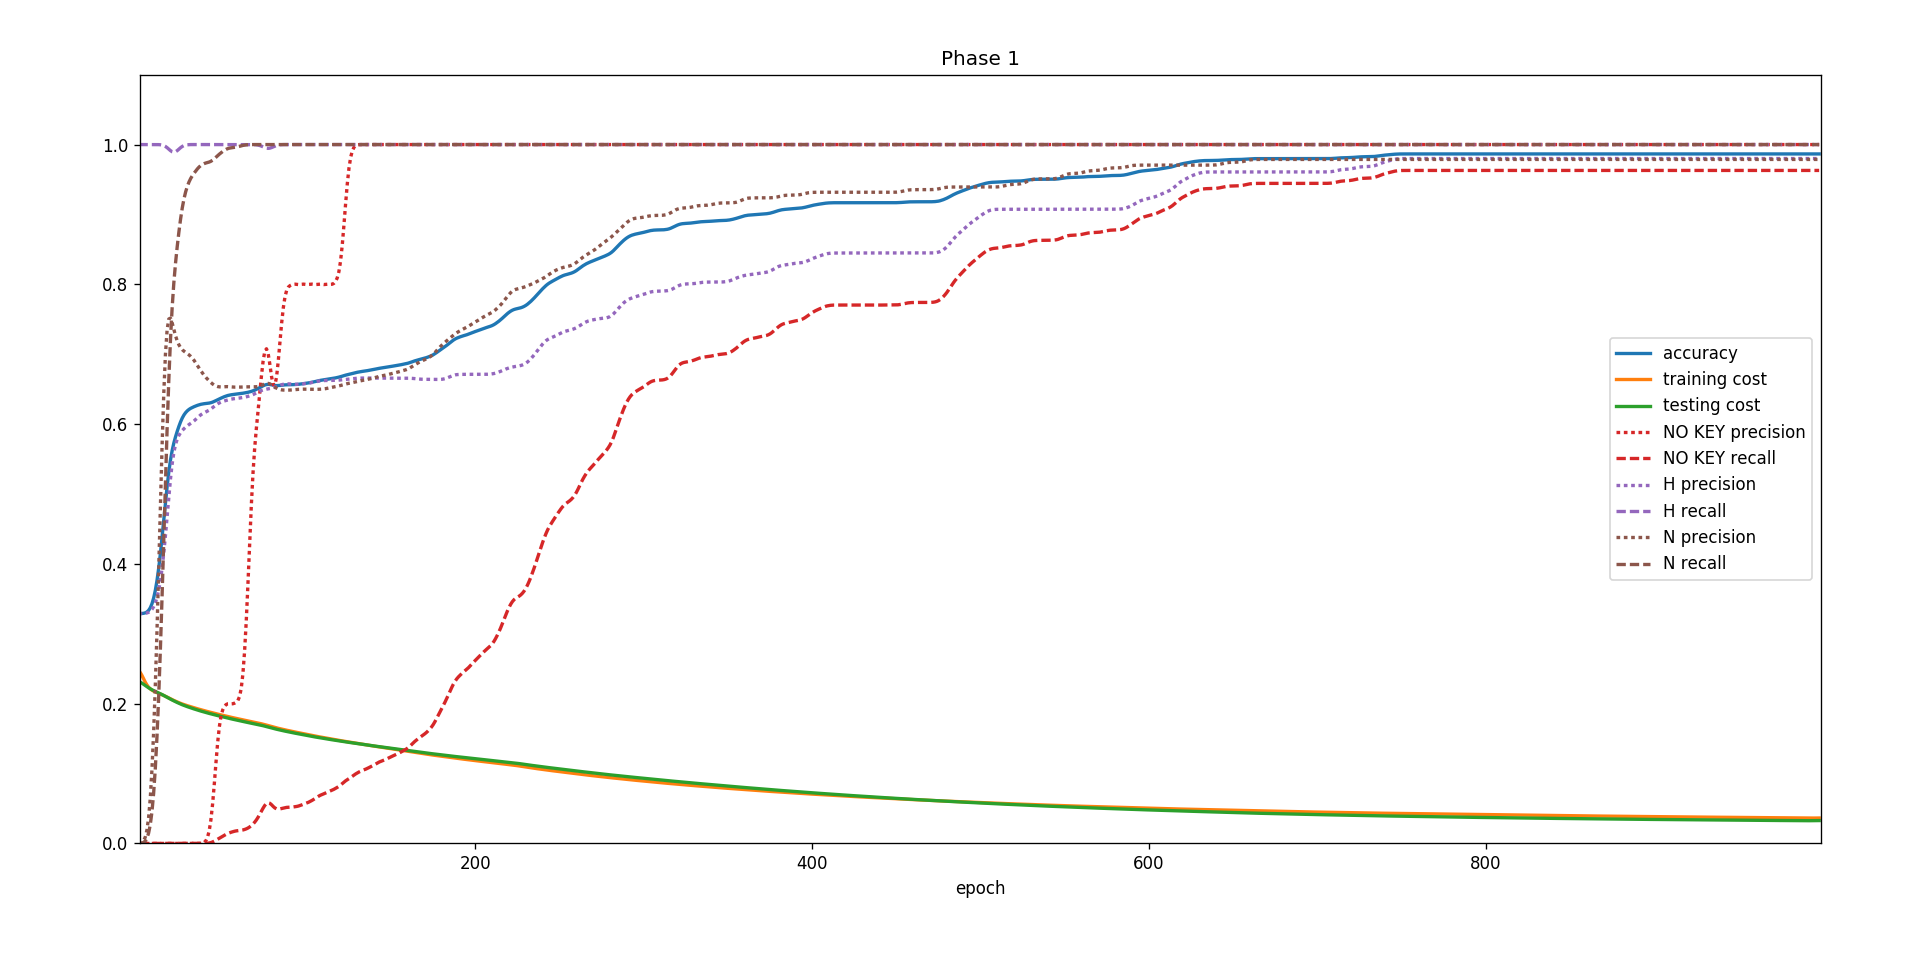
\includegraphics[width=\textwidth]{../common/images/phase-1-detailed}
       \label{fig:phase22}
       \caption{Performance metrics of phase 1, including per key precision and recall}
   \end{figure}
\end{frame}




\cleardoublepage
\thispagestyle{empty}

\vspace*{\fill}
\pagestyle{empty}

{\normalsize
\begin{center}\textbf{Eidesstattliche Erklärung}\end{center}
Hiermit versichere ich an Eides statt, dass ich die vorliegende Arbeit im
Bachelorstudiengang Informatik selbstständig verfasst und keine anderen als die
angegebenen Hilfsmittel -- insbesondere keine im Quellenverzeichnis nicht
benannten Internet-Quellen -- benutzt habe. Alle Stellen, die wörtlich oder
sinngemäß aus Veröffentlichungen entnommen wurden, sind als solche kenntlich
gemacht. Ich versichere weiterhin, dass ich die Arbeit vorher nicht in einem
anderen Prüfungsverfahren eingereicht habe und die eingereichte schriftliche
Fassung der auf dem elektronischen Speichermedium entspricht.
\vspace*{1cm}\\
Hamburg, den 12.06.2017
\hspace*{\fill}\begin{tabular}{@{}l@{}}\hline
\makebox[5cm]{Paul Bienkowski}
\end{tabular}
\vspace*{3cm}
%Dies ist optional, ggf. löschen!
\begin{center}\textbf{Veröffentlichung}\end{center}
Ich stimme der Einstellung der Arbeit in die Bibliothek des Fachbereichs Informatik zu.
\vspace*{1cm}\\
Hamburg, den 12.06.2017
\hspace*{\fill}\begin{tabular}{@{}l@{}}\hline
\makebox[5cm]{Paul Bienkowski}
\end{tabular}
}
\vspace*{\fill}

\end{document}
